\documentclass[%
11pt,%
%oneside,%
twoside,%
%twocolumn,%
titlepage,%
%fleqn,%
%a4page,%
german,%
headsepline%
]{scrartcl}

%\usepackage{fancyhdr}
%\usepackage{scrpage2}
\usepackage{lastpage}
\usepackage{geometry}
\usepackage{graphicx}
\usepackage[utf8]{inputenc}
\usepackage[ngerman]{babel}
\usepackage{lscape}
\usepackage[framemethod=TikZ]{mdframed}
\usepackage[most]{tcolorbox}
\usepackage{mymath}
\usepackage{units}
\usepackage{nicefrac}
\usepackage{pgf,tikz}
\usetikzlibrary{arrows}
\usepackage{colortbl}
\usepackage{hhline}
\usepackage{multirow}
\usepackage[extendedchars]{grffile}
\usepackage{caption}
\usepackage{multicol,calc}
\usepackage{blindtext}
\usepackage{pdfpages}
\usepackage{hyperref}
%\usepackage{tikz-er2}
\usepackage{framed}
\usetikzlibrary{arrows}
\usetikzlibrary{positioning}
\usetikzlibrary{shadows}

%\usepackage{romannum}
\usepackage{longtable}
\usepackage{listings}
\usepackage{wrapfig}

\usepackage{marginnote}
\usepackage{qrcode}
\qrset{height=9ex}

% Command, um Tabellen-Spalten anzupassen
\newcommand{\spaltenheight}{\rule{0mm}{3ex}}
\newcommand{\spaltenwidth}{\rule{3cm}{0mm}}
\newcommand{\spaltensep}{\\[1ex]}
%\arrayrulecolor{darkgreen}
\doublerulesepcolor{white}
\definecolor{lightyellow}{rgb}{1,1,0.8}
\definecolor{Gray}{gray}{0.9}


% Pagestyle/Layout
%\geometry{a4paper , tmargin =2.5cm,	bmargin=3cm, lmargin =2.5cm,	rmargin =2.5cm,	headheight=3em, headsep=1em, footskip=1cm}
\setlength{\parindent}{0pt} \setlength{\parskip}{1em}
%für TwoSide
%\lehead{\headmark\pagemark}
%\cehead{}
%\rehead{}
%\lohead{}
%\cohead{}
%\rohead{\headmark}
%für OneSide
%\ihead{}
%\chead{}
%\ohead{}
%\setheadsepline{0.5pt} % Linie zur Begrenzung
%\setfootsepline{0.5pt} % Linie zur Begrenzung
\pagestyle{headings} % gemachte Einstellungen anwenden

% Farbig umrahmte Umgebung Satz
 
 \definecolor{myblizzardblue}{HTML}{87CEEB}

\newcounter{satzz}[section]\setcounter{satzz}{0}
\renewcommand{\thesatz}{\arabic{section}.\arabic{satzz}}

\newenvironment{csatz}[2][]{%
    \refstepcounter{satzz}
 
    \ifstrempty{#1}%
    % if condition (without title)
    {\mdfsetup{%
        frametitle={%
            \tikz[baseline=(current bounding box.east),outer sep=0pt]
            \node[anchor=east,rectangle,fill=myblizzardblue]
            {\strut Satz~\thesatz};}
        }%
    % else condition (with title)
    }{\mdfsetup{%
        frametitle={%
            \tikz[baseline=(current bounding box.east),outer sep=0pt]
            \node[anchor=east,rectangle,fill=myblizzardblue]
            {\strut Satz~\thesatz:~#1};}%
        }%
    }%
% for both conditions
    \mdfsetup{%
        innertopmargin=10pt,linecolor=myblizzardblue,%
        backgroundcolor=whitesmoke,%
        linewidth=2pt,topline=true,%
        frametitleaboveskip=\dimexpr-\ht\strutbox\relax%
    }
 
\begin{mdframed}[]\relax}{%
\end{mdframed}}

% Farbig umrahmte Umgebung Theorem
 
\definecolor{mygraphblue}{HTML}{84B7E1}
\definecolor{whitesmoke}{HTML}{F5F5F5}

\newcounter{theo}[section]\setcounter{theo}{0}
\renewcommand{\thetheo}{\arabic{section}.\arabic{theo}}

\newenvironment{ctheo}[2][]{%
    \refstepcounter{theo}
 
    \ifstrempty{#1}%
    % if condition (without title)
    {\mdfsetup{%
        frametitle={%
            \tikz[baseline=(current bounding box.east),outer sep=0pt]
            \node[anchor=east,rectangle,fill=mygraphblue]
            {\strut Theorem~\thetheo};}
        }%
    % else condition (with title)
    }{\mdfsetup{%
        frametitle={%
            \tikz[baseline=(current bounding box.east),outer sep=0pt]
            \node[anchor=east,rectangle,fill=mygraphblue]
            {\strut Theorem~\thetheo:~#1};}%
        }%
    }%
% for both conditions
    \mdfsetup{%
        innertopmargin=10pt,linecolor=mygraphblue,%
        backgroundcolor=whitesmoke,%
        linewidth=2pt,topline=true,%
        frametitleaboveskip=\dimexpr-\ht\strutbox\relax%
    }
 
\begin{mdframed}[]\relax}{%
\end{mdframed}}

% Farbig umrahmte Umgebung Definition
 
 \definecolor{emerald}{HTML}{50C878}

\newcounter{deff}[section]\setcounter{deff}{0}
\renewcommand{\thedeff}{\arabic{section}.\arabic{deff}}

\newenvironment{cdef}[2][]{%
    \refstepcounter{deff}
 
    \ifstrempty{#1}%
    % if condition (without title)
    {\mdfsetup{%
        frametitle={%
            \tikz[baseline=(current bounding box.east),outer sep=0pt]
            \node[anchor=east,rectangle,fill=emerald]
            {\strut Definition~\thedeff};}
        }%
    % else condition (with title)
    }{\mdfsetup{%
        frametitle={%
            \tikz[baseline=(current bounding box.east),outer sep=0pt]
            \node[anchor=east,rectangle,fill=emerald]
            {\strut Definition~\thedeff:~#1};}%
        }%
    }%
% for both conditions
    \mdfsetup{%
        innertopmargin=10pt,linecolor=emerald,%
        backgroundcolor=whitesmoke,%
        linewidth=2pt,topline=true,%
        frametitleaboveskip=\dimexpr-\ht\strutbox\relax%
    }
 
\begin{mdframed}[]\relax}{%
\end{mdframed}}

% Farbig umrahmte Umgebung Achtung
 
 \definecolor{mygraphred}{HTML}{E26A6A}

\newcounter{merkee}[section]\setcounter{merkee}{0}
\renewcommand{\themerkee}{\arabic{section}.\arabic{merkee}}

\newenvironment{cachtung}[2][]{%
    \refstepcounter{merkee}
 
    \ifstrempty{#1}%
    % if condition (without title)
    {\mdfsetup{%
        frametitle={%
            \tikz[baseline=(current bounding box.east),outer sep=0pt]
            \node[anchor=east,rectangle,fill=mygraphred]
            {\strut Achtung};}
        }%
    % else condition (with title)
    }{\mdfsetup{%
        frametitle={%
            \tikz[baseline=(current bounding box.east),outer sep=0pt]
            \node[anchor=east,rectangle,fill=mygraphred]
            {\strut Achtung:~#1};}%
        }%
    }%
% for both conditions
    \mdfsetup{%
        innertopmargin=10pt,linecolor=mygraphred,%
        backgroundcolor=whitesmoke,%
        linewidth=2pt,topline=true,%
        frametitleaboveskip=\dimexpr-\ht\strutbox\relax%
    }
 
\begin{mdframed}[]\relax}{%
\end{mdframed}}

\subject{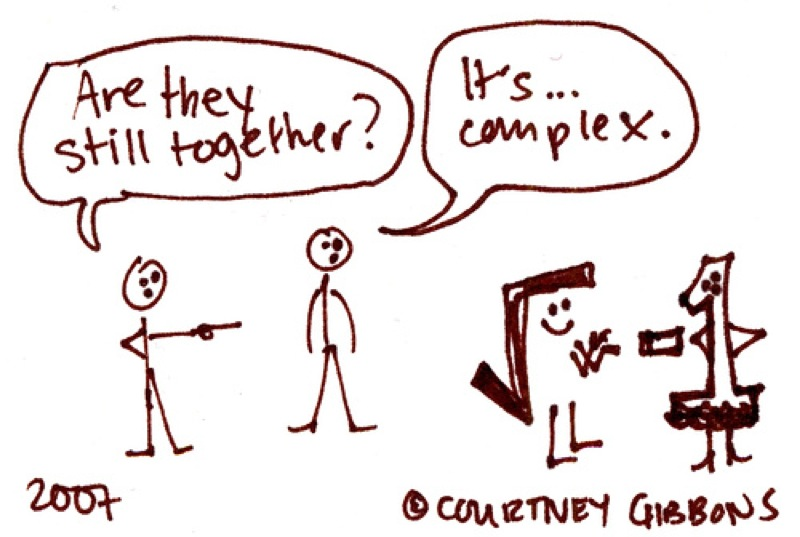
\includegraphics[width=0.618\textwidth]{pictures/itscomplex}}
\title{Komplexe Zahlen}
\subtitle{Vom Unvorstellbaren zum Imaginären}
\author{}
\date{}
%\lowertitleback{
%\includegraphics[height=1.1cm]{/Users/jormawassmer/Pictures/logokoeniz.jpg}%
%\copyright Jorma Wassmer
%1. Auflage, Februar 2011
%}


\begin{document}
\maketitle
\thispagestyle{empty}
\cleardoublepage
\tableofcontents
\cleardoublepage

\pagestyle{headings}

\section{Entdeckung}

Um die Notwendigkeit der imaginären Zahlen besser zu erkennen, scheint es mir sinnvoll, noch einmal auf die Entstehung unserer bereits bekannten Zahlenmengen zur\"uck zu blicken.

In den nat\"urlichen Zahlen $\mN$ kann problemlos addiert werden; das Ergebnis liegt wieder in $\mN$:
$$a,b\in\mN\implies a+b\in\mN.$$
Man sagt, dass die nat\"urlichen Zahlen \textbf{abgeschlossen} bez\"uglich der Addition sind. Ferner sind sie auch abgeschlossen bez\"uglich der Multiplikation.
Will man Abgeschlossenheit bez\"uglich der Subtraktion, so m\"ussen wir unsere Menge mit negativen Zahlen zu den ganzen Zahlen $\mZ$ erweitern, f\"ur eine abgeschlossene Division zu $\mQ$. Die positiven reellen Zahlen sind abgeschlossen bez\"uglich des Potenzierens, d.h. es gilt
$$a\in\mR^+,r\in\mR\implies a^r\in\mR^+.$$
Fordert man schliesslich die Abgeschlossenheit aller reellen Zahlen $\mR$ bez\"uglich des Potenzierens, so stellt sich die Frage, wie man die bislang sinnlosen Ausdr\"ucken
$(-1)^{\frac{1}{2}}$
definieren soll/kann. Damit hätte man eine \glqq Zahl\grqq, welche die Gleichung
$$x^2=-1$$
l\"osen w\"urde.

Die
\marginnote{
\qrcode{
https://www.youtube.com/watch?v=ns42eGJsjjs}
}
komplexen Zahlen stellen eine sinnvolle Erweiterung der reellen Zahlen $\mR$ dar --- genau wie $\mR$ eine Erweiterung der rationalen Zahlen $\mQ$ darstellt, oder $\mQ$ eine Erweiterung der ganzen Zahlen $\mZ$, und diese wiederum eine Erweiterung der nat\"urlichen Zahlen $\mN$.
Erinnern Sie sich, dass Sie viele Probleme erst l\"osen konnten, nachdem Sie die reellen Zahlen kannten? Genauso ist es mit den komplexen Zahlen. Viele Probleme, die in $\mR$ keine L\"osung besitzen, werden im Bereich der komplexen Zahlen endlich l\"osbar. Dar\"uber hinaus erlaubt die geometrische Interpretation der komplexen Zahlen eine elegante Beschreibung von geometrischen Abbildungen und f\"uhrt zu einer Vielzahl neuer Fragestellungen.

\pagebreak

\section{Komplexe Zahlen}
\begin{wrapfigure}{r}{0.48\textwidth}
\vspace{-22pt}
\begin{center}
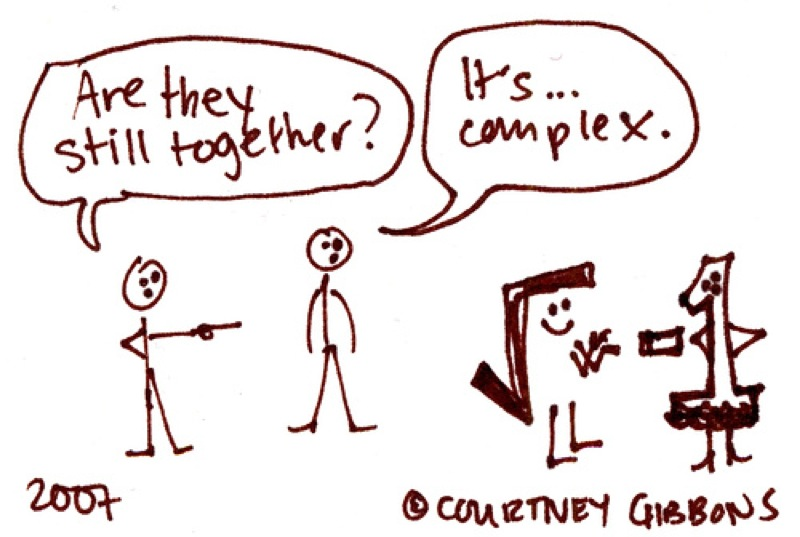
\includegraphics[width=0.48\textwidth]{pictures/itscomplex}
\caption{Imaginäre Zahl}
\end{center}
\end{wrapfigure}
Im Zahlbereich der reellen Zahlen k\"onnen Sie uneingeschränkt alle Ihnen vertrauten Rechenoperationen ausf\"uhren. Alle? Nein! So stossen Sie zum Beispiel beim Wurzelziehen an eine Grenze des Zahlbereichs: Die Gleichung
$$x^2 = -1$$
ist unl\"osbar. Es gibt keine reelle Zahl, deren Quadrat gleich $-1$ ist. Allgemeiner gilt: Quadratische Gleichungen sind manchmal l\"osbar und manchmal nicht.
Um diesen Mangel zu beheben, soll eine neue Zahl eingef\"uhrt werden. Das heisst, der Zahlbereich der reellen Zahlen soll erweitert werden. Ganz ähnlich wurde seinerzeit auch der Zahlbereich $\mQ$ der rationalen Zahlen auf den Bereich $\mR$ der reellen Zahlen erweitert.
Ausgangspunkt war damals die Frage nach der L\"osung der Gleichung
$$x^2 = 2.$$
Diese Gleichung besitzt keine L\"osung in $\mQ$, den rationalen Zahlen. Es gibt keine Bruchzahl, deren Quadrat gleich $2$ ist. Deshalb wurde eine neue Zahl eingef\"uhrt, welche die Gleichung $x^2 = 2$ l\"osbar macht. Sie wurde mit $\sqrt{2}$ bezeichnet und hat die Eigenschaft, dass sie mit sich selbst multipliziert $2$ ergibt:
$$\sqrt{2}\cdot\sqrt{2}=2.$$

\subsection{Das Permanenzprinzip}

Auf diese Weise wurde der Zahlbereich $\mQ$ der rationalen Zahlen erweitert. Es entstand der weitaus umfassendere Zahlbereich $\mR$ der reellen Zahlen, der unter anderem auch alle Wurzeln enthält. Bei dieser Erweiterung von $\mQ$ nach $\mR$ wurden drei wesentliche Punkte eingehalten:

\begin{enumerate}
\item Die alten Zahlen sind ein Teil der neuen Zahlen. So sind beispielsweise die rationalen Zahlen eine Teilmenge der reellen Zahlen. Mit Symbolen ausgedr\"uckt schreiben wir das als $\mQ\subset\mR$.
\item Alle Rechenoperationen, die mit den alten Zahlen m\"oglich sind, sind auch mit den neuen Zahlen m\"oglich. Die Erweiterung von den rationalen Zahlen zu den reellen Zahlen erzeugt keine Einschränkungen.
\item F\"ur die neuen Zahlen gelten dieselben Rechenregeln wie f\"ur die alten. So k\"onnen Sie mit den reellen Zahlen genauso rechnen wie mit den rationalen Zahlen.
\end{enumerate}

Es ist vern\"unftig, dieses \textbf{Permanenzprinzip} bei der Erweiterung eines Zahlbereichs zu fordern. Denn wir wollen so wichtige Eigenschaften wie die G\"ultigkeit der Rechenregeln nicht verlieren.

\subsection{Die imaginäre Einheit i}

In $\mR$ ist die Gleichung
$$x^2=-1$$
nicht l\"osbar, da das Quadrat einer von Null verschiedenen reellen Zahl stets positiv ist.

Wir wollen den Bereich der reellen Zahlen nun so erweitern, dass die Gleichung $x^2 = -1$ l\"osbar ist. Dazu f\"uhren wir eine neue Zahl ein, welche diese Gleichung l\"osbar macht. Diese neue Zahl nennen wir \textbf{imagin\"are Einheit}
und bezeichnen sie mit dem Symbol $\mathrm{i}$. Sie soll die Eigenschaft haben, dass sie mit sich selbst multipliziert $-1$ ergibt:
$$\mathrm{i}\cdot \mathrm{i} = -1.$$
Was k\"onnen wir uns nun unter diesem $i$ vorstellen? Mit Sicherheit ist $\mathrm{i}$ keine reelle Zahl, denn wie oben bereits gesagt, ist das Quadrat einer reellen Zahl niemals negativ. Es gilt aber $\mathrm{i}^2 = -1$, denn wir haben ja gefordert, dass $\mathrm{i}$ eine L\"osung der Gleichung $x^2 = -1$ sein soll.
Wir wissen also nicht, wie $\mathrm{i}$ \glqq aussieht\grqq. Wir k\"onnen aber bereits mit $\mathrm{i}$ rechnen.

\begin{bsp}
Nach dem dritten Punkt des Permanenzprinzips sollen die Rechenregeln aus $\mR$ ja weiterhin g\"ultig sein. So k\"onnen wir zum Beispiel $\mathrm{i}^3$ berechnen:
$$\mathrm{i}^3=\mathrm{i}^2\cdot \mathrm{i}=(-1)\cdot \mathrm{i}=-\mathrm{i}.$$
\end{bsp}

\begin{ueb}[Rechne mit $\mathrm{i}$]
Berechne

\begin{minipage}{0.3\textwidth}
\begin{enumeratea}
\item $\mathrm{i}^2$
\item $\mathrm{i}^4$
\item $\mathrm{i}^5$
\end{enumeratea}
\end{minipage}
\begin{minipage}{3.5cm}
\begin{enumeratea}
\setcounter{enumi}{3}
\item $(-\mathrm{i})^2$
\item $-\mathrm{i}^2$
\item $-\mathrm{i}^4$
\end{enumeratea}
\end{minipage}
\end{ueb}

Fr\"uheren Mathematikern war die Zahl $\mathrm{i}$ \"ubrigens etwas unheimlich. \textsc{Gottfried Wilhelm Leibniz} (1646-1716) beispielsweise nannte sie \glqq ein Amphibium zwischen Sein und Nicht-sein\grqq, f\"ur \textsc{Leonhard Euler} (1707-1783) war sie eine \glqq unm\"ogliche Zahl\grqq, und noch \textsc{Carl Friedrich Gauss} (1777-1855) bezeichnete sie im neunzehnten Jahrhundert als \glqq Schatten von Schatten\grqq.
Da $\mathrm{i}$ also eine \glqq unm\"ogliche Zahl\grqq\ war, das heisst keine reelle Zahl, nannte man sie \emph{imagin\"ar} (von lateinisch imaginarius = eingebildet). Die Bezeichnung geht auf René Descartes (1596-1650) zur\"uck.

\begin{cdef}[Imaginäre Einheit]{def:i}
Die Zahl $\mathrm{i}$ mit
$$\mathrm{i}^2=-1$$
heisst \emph{imagin\"are Einheit}.
\end{cdef}

\begin{figure}
\begin{center}
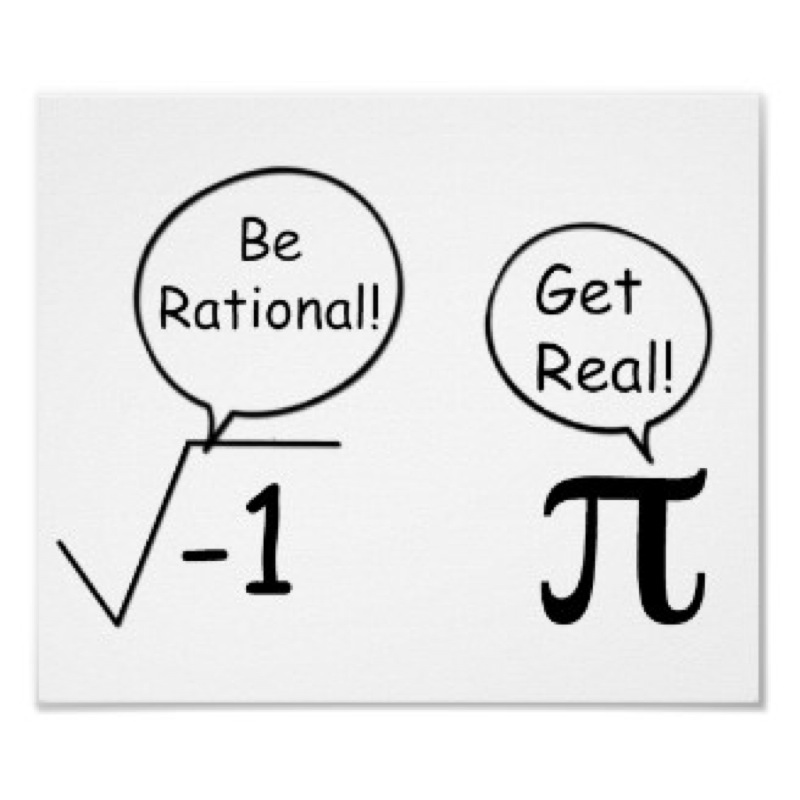
\includegraphics[width=0.38\textwidth]{pictures/getreal}
\caption{$\pi$ and $i$}
\end{center}
\end{figure}

\subsection{Komplexe Zahlen}

Nachdem wir nun die imagin\"are Einheit $\mathrm{i}$ kennen gelernt haben, wollen wir diese mit den reellen Zahlen verkn\"upfen. Dazu bilden wir die so genannten \textbf{komplexen Zahlen}. Das Wort komplex steht hier f\"ur \glqq zusammengesetzt\grqq\ (von lateinisch complexus: verflochten).

\begin{bsp}
$$1+3\mathrm{i},\q -1+3\mathrm{i},\q 2-5\mathrm{i},\q \frac{3}{4}+7\mathrm{i},\q -\sqrt{3}+\pi \mathrm{i}$$
sind komplexe Zahlen. Sie alle sind zusammengesetzt aus einem reellen Anteil (bei $1 + 3\mathrm{i}$ ist das beispielsweise $1$) und einem imagin\"aren Anteil (bei $1 + 3\mathrm{i}$ ist das beispielsweise $3\mathrm{i}$).
\end{bsp}

\begin{cdef}[Komplexe Zahl]{def:komplex}
Eine Zahl $z$ der Form
$$z=a+b\mathrm{i}$$
heisst \emph{komplexe Zahl}. $a$ und $b$ sind dabei reelle Zahlen. $\mathrm{i}$ steht f\"ur die imaginäre Einheit.
\end{cdef}

Wir betrachten noch einmal die komplexe Zahl $2 -5\mathrm{i}$. Bei dieser Zahl spielen offensichtlich die $2$ und die $-5$ eine besondere Rolle. Wenn Ihnen jemand sagt: \glq Bei der komplexen Zahl $z$ ist der rein reelle Anteil $2$, und vor der imaginären Einheit steht $-5$\grqq, dann wissen Sie genau, um welche komplexe Zahl es sich handelt; es kann nur $2-5\mathrm{i}$ sein. Jede komplexe Zahl $a+b\mathrm{i}$ ist durch die reellen Zahlen $a$ und $b$ eindeutig festgelegt.
Um komplexe Zahlen auf diese Art beschreiben zu k\"onnen, f\"uhren wir zwei neue Begriffe ein:
Unter dem \emph{Realteil} einer komplexen Zahl wollen wir in Zukunft den rein reellen Anteil der Zahl verstehen. Der Realteil der komplexen Zahl $2 - 5\mathrm{i}$ ist also $2$. Wir schreiben auch $\re(2 - 5\mathrm{i}) = 2$.
Unter dem \emph{Imagin\"arteil} einer komplexen Zahl wollen wir in Zukunft den Teil der Zahl verstehen, der vor der imaginären Einheit $\mathrm{i}$ steht. Der Imaginärteil der komplexen Zahl $2 -5\mathrm{i}$ ist also $-5$. Wir schreiben auch $\im(2 - 5\mathrm{i}) = -5$.

\begin{ueb}[Re und Im]
Gib Realteil und Imaginärteil der folgenden komplexen Zahlen an. Verwende dazu die Schreibweisen $\re$ und $\im$. (Schreibe also beispielsweise $\re(3 + 2\mathrm{i}) = 3$, $\im(3 + 2\mathrm{i}) = 2$.)

\begin{minipage}{0.3\textwidth}
\begin{enumeratea}
\item $-1+4\mathrm{i}$
\item $2-5\mathrm{i}$
\item $\frac{3}{4}+7\mathrm{i}$
\item $\sqrt{7}+\frac{5}{6}\mathrm{i}$
\end{enumeratea}
\end{minipage}
\begin{minipage}{0.4\textwidth}
\begin{enumeratea}
\setcounter{enumi}{4}
\item $\sqrt{5}\mathrm{i}$
\item $-\frac{1}{6}$
\item $\mathrm{i}$
\item $0$
\end{enumeratea}
\end{minipage}
\end{ueb}

Zum Schluss halten wir die Definitionen der neuen Begriffe noch einmal fest.

\begin{cdef}[Real- und Imaginärteil]{def:reim}
Es sei
$$z=a+b\mathrm{i}$$
mit $a,b\in\mR$ eine komplexe Zahl. Dann heisst $a$ der \emph{Realteil} und $b$ der \emph{Imagin\"arteil} von $z$. Man schreibt $\re(z)=a$ bzw. $\im(z)=b$.
\end{cdef}

\begin{ueb}[Re plus Im]
F\"ur welche komplexen Zahlen $z$ gilt
$$z=\re(z)+\im(z)?$$
\end{ueb}

\begin{ueb}[Re von Im]
F\"ur welche Zahlen $z$ gilt
$$\re(\im(z))=0?$$
\end{ueb}

\begin{bem}
Man beachte, dass sowohl der Realteil als auch der Imagin\"arteil einer komplexen Zahl $z$ reell sind. Zahlen der Form $b\mathrm{i}$ heissen \emph{rein imaginär}.
\end{bem}

\subsection{Die komplexen Zahlen sind eine Erweiterung der reellen Zahlen}

Im vorigen Abschnitt haben wir gesehen, dass wir f\"ur die reelle Zahl $-\frac{1}{6}$ auch als komplexe Zahl $-\frac{1}{6}+0\mathrm{i}$ auffassen k\"onnen. Die reellen Zahlen sind gerade die komplexen Zahlen mit Imaginärteil $0$. In andern Worten: Die reellen Zahlen $\mR$ sind eine Teilmenge der komplexen Zahlen, f\"ur die \"ublicherweise die Abk\"urzung $\mC$ verwendet wird.

\begin{bem}
Die Menge der komplexen Zahlen bezeichnen wir mit $\mC$. Es gilt
$$\mR\subset\mC.$$
\end{bem}

\begin{ueb}[Zahlenmengen]
Zu welchen Mengen $\mN,\mZ,\mQ,\mR,\mC$ geh\"oren die Zahlen

\begin{minipage}{0.3\textwidth}
\begin{enumeratea}
\item $2$
\item $-\sqrt{3}$
\item $3+\frac{1}{2}\mathrm{i}$
\end{enumeratea}
\end{minipage}
\begin{minipage}{0.4\textwidth}
\begin{enumeratea}
\setcounter{enumi}{3}
\item $0$
\item $4\mathrm{i}$
\item $\mathrm{i}^8$
\end{enumeratea}
\end{minipage}
\end{ueb}

\section{Wie rechnet man mit komplexen Zahlen?}
\subsection{Addition und Subtraktion}

Wir betrachten die Addition von komplexen Zahlen an einem Beispiel.

\begin{bsp}
Wir m\"ochten $3+\mathrm{i}$ und $1-2\mathrm{i}$ addieren:
$$(3+\mathrm{i})+(1-2\mathrm{i}).$$
Nach dem Permanenzprinzip sollen die Rechenregeln aus $\mR$ weiterhin g\"ultig sein. Wie w\"urden Sie im Reellen addieren, wenn $i$ eine Variable wäre? Ganz klar, Sie w\"urden die beiden rein reellen Ausdr\"ucke (d.h. die $3$ und die $1$) zusammenfassen, und ebenso die beiden rein imaginären Ausdr\"ucke (d.h. $\mathrm{i}$ und $-2\mathrm{i}$). Das Gleiche tun wir auch hier. Wir schreiben
$$
(3+\mathrm{i})+(1-2\mathrm{i})=3+\mathrm{i}+1-2\mathrm{i}=(3+1)+(\mathrm{i}-2\mathrm{i})=4-\mathrm{i}.
$$
\end{bsp}

\begin{bem}
Bei der Subtraktion funktioniert das Zusammenfassen der rein reellen Ausdr\"ucke und der rein imaginären Ausdr\"ucke analog.
\end{bem}

\begin{ueb}[subtrahieren]
Berechne $(3+\mathrm{i})-(1-2\mathrm{i})$.
\end{ueb}

\begin{ueb}[addieren und subtrahieren]
Berechne

\begin{minipage}{0.4\textwidth}
\begin{enumeratea}
\item $(4+3\mathrm{i})+(2+\mathrm{i})$
\item $(\frac{1}{4}+2\mathrm{i})+(\frac{1}{5}-\mathrm{i})$
\item $(\sqrt{5}+3\mathrm{i})+(-2+\mathrm{i})-(4\mathrm{i})$
\end{enumeratea}
\end{minipage}
\begin{minipage}{0.4\textwidth}
\begin{enumeratea}
\setcounter{enumi}{3}
\item $(4+3\mathrm{i})-(2+3\mathrm{i})$
\item $\re((-2+\mathrm{i})-(-2-3\mathrm{i}))$
\item $\im(7-(4+3\mathrm{i})-(5-4\mathrm{i}))$
\end{enumeratea}
\end{minipage}
\end{ueb}

\begin{ueb}[mission impossible]
Lässt sich $1$ als Summe von zwei rein imaginären Zahlen schreiben?
\end{ueb}

\pagebreak

\begin{cdef}[Addition]{def:add}
Die Summe bzw. Differenz zweier komplexer Zahlen $a+b\mathrm{i}$ und $c+d\mathrm{i}$ erfolgt komponentenweise, indem man die Realteile und die Imaginärteile separat addiert bzw. subtrahiert. Es gilt
$$(a+b\mathrm{i})+(c+d\mathrm{i})=(a+c)+(b+d)\mathrm{i}$$
bzw.
$$(a+b\mathrm{i})-(c+d\mathrm{i})=(a-c)+(b-d)\mathrm{i}$$
\end{cdef}

\subsection{Multiplikation}

Wir multiplizieren zwei komplexe Zahlen miteinander.

\begin{bsp}
Nach dem Permanenzprinzip muss zum Beispiel
$$(3+\mathrm{i})\cdot(1-2\mathrm{i})=3-6\mathrm{i}+\mathrm{i}-2\mathrm{i}^2$$
gelten. Nach Definition von $\mathrm{i}^2=-1$ folgt
$$3-6\mathrm{i}+\mathrm{i}-2\mathrm{i}^2=3-5\mathrm{i}-(-2)=5-5\mathrm{i}.$$
\end{bsp}

\begin{ueb}[multiplication rule]
Berechne f\"ur $v=1+\mathrm{i}$, $w=4\mathrm{i}$ und $z=2-5\mathrm{i}$ die Ausdr\"ucke

\begin{minipage}{0.3\textwidth}
\begin{enumeratea}
\item $v\cdot z$
\item $v(w-z)$
\end{enumeratea}
\end{minipage}
\begin{minipage}{3.5cm}
\begin{enumeratea}
\setcounter{enumi}{2}
\item $\re(vwz)$
\item $\im(v+wz)$
\end{enumeratea}
\end{minipage}
\end{ueb}

\begin{ueb}[swap]
Wahr oder falsch: Wird eine komplexe Zahl mit $(-\mathrm{i})$ multipliziert, dann werden Real- und Imaginärteil vertauscht.
\end{ueb}

Wir halten fest:

\begin{csatz}[Multiplikation]{satz:mul}
Sind $a+b\mathrm{i}$ und $c+d\mathrm{i}$ zwei komplexe Zahlen, dann gilt
$$(a+b\mathrm{i})\cdot(c+d\mathrm{i})=(ac-bd)+(ad+bc)\mathrm{i}.$$
\end{csatz}

\begin{proof}[Beweis]
easy
\end{proof}

Leider ist die Regel f\"ur die Multiplikation nicht so einfach wie f\"ur die Addition und Subtraktion, wo Real- und Imaginärteile separat addiert werden.

\begin{ueb}[Produkt]
Zeige: Im Allgemeinen gilt nicht $\re(z\cdot w)=\re(z)\cdot\re(w)$.
\end{ueb}

\subsection{Konjugiert komplexe Zahlen}

Bevor wir uns die Division von komplexen Zahlen genauer ansehen, f\"uhren wir einen neuen Begriff ein. Jede komplexe Zahl besitzt eine so genannte \emph{konjugiert komplexe Zahl}. Dieser Begriff wird sich bei der Division als sehr n\"utzlich erweisen, und er wird in späteren Kapiteln ebenfalls immer wieder von Bedeutung sein.

\begin{bsp}
Als Beispiel betrachten wir die Zahl $5 + 3\mathrm{i}$. Die zu $5 + 3\mathrm{i}$ konjugiert komplexe Zahl ist $5- 3\mathrm{i}$. Die Realteile der beiden Zahlen sind gleich, die Imaginärteile der beiden Zahlen sind entgegengesetzt gleich, d.h. sie unterscheiden sich nur durch das Vorzeichen.
\end{bsp}

†berraschend ist nun das Produkt der beiden Zahlen.

\begin{ueb}[konjugiert komplex]
Berechne $(5+3\mathrm{i})\cdot(5-3\mathrm{i})$.
\end{ueb}

\begin{bem}
Das Produkt der beiden konjugiert komplexen Zahlen ist reell! Dies ist die bedeutendste Eigenschaft konjugiert komplexer Zahlen und wird sich immer wieder als n\"utzlich erweisen.
\end{bem}

\begin{cdef}[Konjugiert komplex]{def:conj}
Es sei $z=a+b\mathrm{i}$ eine komplexe Zahl. Die zu $z$ \emph{konjugiert komplexe Zahl} ist die Zahl
$$a-b\mathrm{i}.$$
Man schreibt daf\"ur auch $\bar{z}$. (lies: \glqq $z$ bar\grqq)
\end{cdef}

\begin{ueb}[rechne]
Seien $w=3\mathrm{i}$ und $z=\frac{1}{2}+4\mathrm{i}$. Berechne

\begin{minipage}{3.5cm}
\begin{enumeratea}
\item $\bar{z}$
\item $\overline{w}$
\end{enumeratea}
\end{minipage}
\begin{minipage}{3.5cm}
\begin{enumeratea}
\setcounter{enumi}{2}
\item $\overline{w+z}$
\item $\overline{w^2-z}$
\end{enumeratea}
\end{minipage}
\end{ueb}

\begin{ueb}[$z$ bar]
Zeige, dass f\"ur f\"ur alle komplexen Zahlen $z$ gilt:
\begin{enumeratea}
\item $z\cdot \bar{z}=\re(z)^2+\im(z)^2$
\item $z+\bar{z}=2\re(z)$
\item $\bar{\bar{z}}=z$
\end{enumeratea}
\end{ueb}

\begin{ueb}[Achsen]
Welche Zahlen sind durch die Gleichung $z+\bar{z}=0$ festgelegt? Welche Zahlen erf\"ullen $z-\bar{z}=0$?
\end{ueb}

\subsection{Division}

Beispielsweise m\"ochten wir $3+\mathrm{i}$ durch $1-2\mathrm{i}$ teilen. Gesucht ist also
$$(3+\mathrm{i})\div(1-2\mathrm{i})=\frac{3+\mathrm{i}}{1-2\mathrm{i}}.$$
Nach dem Permanenzprinzip sollen die Rechenregeln aus $\mR$ weiterhin g\"ultig sein.

Zunächst einmal st\"ort, dass im Nenner des Bruchs $\mathrm{i}$ vorkommt. Durch eine
reelle Zahl, z.B. 5 zu teilen wäre nämlich ganz einfach:
$$(3+\mathrm{i})\div5=(3+\mathrm{i})\cdot\frac{1}{5}=\frac{3}{5}+\frac{1}{5}\mathrm{i}.$$
Die Frage lautet also: Wie lässt sich aus dem Nenner $1-2\mathrm{i}$ eine reelle Zahl herstellen?

Wir benutzen die Tatsache, dass eine Zahl mal ihr konjugiert Komplexes eine reelle Zahl ergibt und erweitern also den Bruch mit der zu $1 - 2\mathrm{i}$ konjugiert komplexen Zahl $1 + 2\mathrm{i}$. Dadurch wird der Nenner reell; das $\mathrm{i}$ \glqq verschwindet\grqq. Im Zähler entsteht zwar ein Produkt von komplexen Zahlen, das man aber durch Multiplizieren leicht berechnen kann. In der Tat:
$$\frac{3+\mathrm{i}}{1-2\mathrm{i}}=\frac{(3+\mathrm{i})(1+2\mathrm{i})}{(1-2\mathrm{i})(1+2\mathrm{i})}=\frac{1+7\mathrm{i}}{5}=\frac{1}{5}+\frac{7}{5}\mathrm{i}.$$

\begin{ueb}[Division]
Berechne die folgenden Ausdr\"ucke

\begin{minipage}{3.5cm}
\begin{enumeratea}
\item $\frac{3+2\mathrm{i}}{7-\mathrm{i}}$
\item $\frac{\mathrm{i}}{-4-4\mathrm{i}}$
\end{enumeratea}
\end{minipage}
\begin{minipage}{3.5cm}
\begin{enumeratea}
\setcounter{enumi}{2}
\item $\frac{1}{\mathrm{i}}$
\item $\frac{3+4\mathrm{i}}{-\mathrm{i}}$
\end{enumeratea}
\end{minipage}
\end{ueb}

\begin{csatz}[Division]{satz:div}
Sind $a+b\mathrm{i}$ und $c+d\mathrm{i}$ zwei komplexe Zahlen und $c+d\mathrm{i}\neq0$, dann gilt
$$(a+b\mathrm{i})\div(c+d\mathrm{i})=\frac{(ac+bd)+(bc-ad)\mathrm{i}}{c^2+d^2}.$$
\end{csatz}

\begin{proof}[Beweis]
Einfache Rechnung
\end{proof}

Damit kennen wir nun alle vier Grundrechenarten mit komplexen Zahlen.

\begin{ueb}[Die vier Grundrechenarten]
Berechne f\"ur $v=5\mathrm{i}$, $w=3-2\mathrm{i}$ und $z=6+4\mathrm{i}$ die folgenden Ausdr\"ucke

\begin{minipage}{3.5cm}
\begin{enumeratea}
\item $z^2-vw$
\item $\frac{z-w}{z+w}$
\end{enumeratea}
\end{minipage}
\begin{minipage}{3.5cm}
\begin{enumeratea}
\setcounter{enumi}{2}
\item $\re(zw(z+v))$
\item $\overline{\left(\frac{vw}{z}\right)}$
\end{enumeratea}
\end{minipage}
\end{ueb}

\clearpage

\section{Die geometrische Darstellung der komplexen Zahlen}

Mit komplexen Zahlen kann man grundsätzlich rechnen wie mit reellen Zahlen. Man kann mit ihnen alle quadratischen Gleichungen l\"osen. Aber das ist bei weitem nicht alles: Komplexe Zahlen und ihre Operationen lassen sich auch geometrisch darstellen. Mit der geometrischen Darstellung der komplexen Zahlen kann man neue Zusammenhänge erkennen, die das L\"osen weiterf\"uhrender Fragen erm\"oglichen.

\subsection{Die Gauss'sche Zahlenebene}

Wir haben komplexe Zahlen definiert als Zahlen der Form
$z = a + b\mathrm{i}$,
wobei $\mathrm{i}$ die imaginäre Einheit ist, und $a$ und $b$ reelle Zahlen sind.
Jede komplexe Zahl $z$ ist also durch ein reelles Zahlenpaar $\point{a}{b}$ eindeutig festgelegt, und umgekehrt geh\"ort zu jeder komplexen Zahl $z$ ein reelles Zahlenpaar $\point{a}{b}$.
Daher liegt es nahe, die geometrische Darstellung komplexer Zahlen in einer Ebene zu manifestieren.

\begin{cdef}[Gauss'sche Zahlenebene]{}
Jeder komplexen Zahl $z=a+b\mathrm{i}$ wird der Punkt $\point{a}{b}$ in der Zahlenebene zugeordnet. Diese Ebene heisst \emph{Gauss'sche Zahlenebene}. Die waagrechte Achse nennt man \emph{reelle Achse}. Die senkrechte Achse heisst \emph{imagin\"are Achse}. Der Koordinatenursprung heisst \emph{Nullpunkt}.
\end{cdef}

\begin{bem}
Die komplexe Ebene wird zu Ehren von \textsc{Carl Friedrich Gauss} (1777-1855) \emph{Gauss'sche Zahlenebene} genannt. Erst C.F. Gauss verhalf der Veranschaulichung dieser fr\"uher unvorstellbaren Zahlen zum Durchbruch und verschaffte ihnen bei Mathematikerinnen und Mathematikern volle Anerkennung.
\end{bem}

\noindent Offensichtlich entspricht die reelle Achse allen reellen Zahlen (also dem urspr\"unglichen Zahlenstrahl) und die imaginäre Achse allen rein imaginären Zahlen.
\begin{figure}
\centering
\vspace{-15pt}
\definecolor{xdxdff}{rgb}{0.49,0.49,1}
\definecolor{qqqqff}{rgb}{0,0,1}
\begin{tikzpicture}[line cap=round,line join=round,>=triangle 45,x=0.8cm,y=0.8cm]
\draw[->,color=black] (-1,0) -- (6.77,0);
\foreach \x in {,1,2,3,4,5,6}
\draw[shift={(\x,0)},color=black] (0pt,2pt) -- (0pt,-2pt);
\draw[color=black] (6.05,0.13) node [anchor=south west] { Re};
\draw[->,color=black] (0,-1.46) -- (0,5.25);
\foreach \y in {-1,1,2,3,4,5}
\draw[shift={(0,\y)},color=black] (2pt,0pt) -- (-2pt,0pt);
\draw[color=black] (0.14,4.61) node [anchor=west] { Im};
\clip(-1,-1.46) rectangle (6.77,5.25);
\draw [dash pattern=on 4pt off 4pt] (0,3)-- (4,3);
\draw [dash pattern=on 4pt off 4pt] (4,3)-- (4,0);
\draw (-0.54,1.37) node[anchor=north west] {$\mathrm{i}$};
\draw (0.75,-0.2) node[anchor=north west] {$1$};
\begin{scriptsize}
\fill [color=qqqqff] (4,3) circle (1.5pt);
\draw[color=qqqqff] (4.24,3.41) node {$a+b\mathrm{i}$};
%\fill [color=xdxdff] (0,3) circle (1.5pt);
\draw[color=xdxdff] (-0.45,3.1) node {$b$};
%\fill [color=qqqqff] (4,0) circle (1.5pt);
\draw[color=qqqqff] (4,-0.41) node {$a$};
\end{scriptsize}
\end{tikzpicture}
\caption{Die Gauss'sche Zahlenebene $\mC$}
\end{figure}

So liegt zum Beispiel die Zahl $1$ eine Einheit rechts des Nullpunkts auf der reellen Achse und die Zahl $\mathrm{i}$ eine Einheit oberhalb des Nullpunkts auf der imaginären Achse.

\begin{ueb}[Argand Diagramm]
Zeichne die folgenden komplexen Zahlen  in die Gauss'\-sche Zahlenebene.

\begin{minipage}{3.5cm}
\begin{enumeratea}
\item $3\mathrm{i}$
\item $-2-\mathrm{i}$
\end{enumeratea}
\end{minipage}
\begin{minipage}{3.5cm}
\begin{enumeratea}
\setcounter{enumi}{2}
\item $3$
\item $3-2\mathrm{i}$
\end{enumeratea}
\end{minipage}
\end{ueb}

\begin{ueb}[oder Gauss'sche Zahlenebene]
Wie lauten die dargestellten Zahlen $u,v,w$?
\begin{center}
\definecolor{qqqqff}{rgb}{0,0,1}
\definecolor{cqcqcq}{rgb}{0.75,0.75,0.75}
\scalebox{0.8}{
\begin{tikzpicture}[line cap=round,line join=round,>=triangle 45,x=0.7cm,y=0.7cm]
\draw [color=cqcqcq,dash pattern=on 4pt off 4pt, xstep=0.7cm,ystep=0.7cm] (-4.33,-4.7) grid (4.64,4.74);
\draw[->,color=black] (-4.33,0) -- (4.64,0);
\foreach \x in {-4,-3,-2,-1,1,2,3,4}
\draw[shift={(\x,0)},color=black] (0pt,2pt) -- (0pt,-2pt) node[below] {\footnotesize $\x$};
\draw[color=black] (3.92,0.13) node [anchor=south west] { Re};
\draw[->,color=black] (0,-4.7) -- (0,4.74);
\foreach \y in {-4,-3,-2,-1,1,2,3,4}
\draw[shift={(0,\y)},color=black] (2pt,0pt) -- (-2pt,0pt) node[left] {\footnotesize $\y \mathrm{i}$};
\draw[color=black] (0.14,4.11) node [anchor=west] { Im};
\draw[color=black] (0pt,-10pt) node[right] {\footnotesize $0$};
\clip(-4.33,-4.7) rectangle (4.64,4.74);
\begin{scriptsize}
\fill [color=qqqqff] (-3,1) circle (1.5pt);
\draw[color=qqqqff] (-2.78,1.4) node {$v$};
\fill [color=qqqqff] (3,0) circle (1.5pt);
\draw[color=qqqqff] (3.2,0.42) node {$u$};
\fill [color=qqqqff] (0,-2) circle (1.5pt);
\draw[color=qqqqff] (0.24,-1.58) node {$w$};
\end{scriptsize}
\end{tikzpicture}
}
\end{center}
\end{ueb}

\begin{ueb}[minus und bar]
Welche geometrische Abbildung in der Gauss'schen Zahlenebene entspricht dem Bilden der entgegengesetzten Zahl $-z$, bzw. dem Bilden der konjugiert komplexen Zahl $\bar{z}$?
\end{ueb}

\begin{bem}
Die entgegengesetzte Zahl $-w$ zu $w$, bzw. die konjugiert komplexe Zahl $\bar{z}$ zu $z$ spielt beim L\"osen von quadratischen Gleichungen eine wichtige Rolle. Mit $w$ ist stets auch $-w$ eine L\"osung von $w^2 = D$, auch wenn die Diskriminante $D$ nicht reell ist. Denn es ist $(-w)^2 = w^2 = D$. Ist $z$ eine nicht reelle L\"osung der quadratischen Gleichung $az^2 + bz + c = 0$ mit reellen Koeffizienten $a, b, c$, dann ist stets auch $\bar{z}$ eine L\"osung dieser Gleichung. Dies geht aus der L\"osungsformel hervor. Nicht reelle L\"osungen einer quadratischen Gleichung mit reellen Koeffizienten liegen in der Gauss'schen Zahlenebene symmetrisch bez\"uglich der reellen Achse.
\end{bem}

\subsection{Die Addition in der Gauss'schen Zahlenebene}

Komplexe Zahlen werden addiert, indem man die Real- und die Imaginärteile separat addiert.

\begin{ueb}[geometrisch addieren]
Gegeben seien die komplexen Zahlen $z_1=3+\mathrm{i}$ und $z_2=1+2\mathrm{i}$.
\begin{enumeratea}
\item Zeichne $z_1, z_2$ und $z_1+z_2$ ein und verbinde die entsprechenden Punkte jeweils mit dem Nullpunkt.
\item Interpretiere das Addieren von $z_1$ mit $z_2$ geometrisch.
\end{enumeratea}
\end{ueb}
\noindent Jedem Zahlenpaar $\point{a}{b}$ lässt sich aber eindeutig der (Orts-)Vektor
$$\pv{a}{b}$$
zuordnen. Wir k\"onnen also jeder komplexen Zahl eindeutig einen Vektor in der Gauss'\-schen Zahlenebene zuordnen. Dieser Vektor kann dargestellt werden durch den Pfeil mit dem Anfangspunkt $0$ und dem Endpunkt $z$.

Der Addition zweier komplexer Zahlen $z_1 = a_1 +b_1\mathrm{i}$ und $z_2 = a_2 +b_2\mathrm{i}$ entspricht in der Gauss'\-schen Zahlenebene die Vektoraddition der zugeh\"origen Vektoren
$$\pv{a_1}{b_1}+\pv{a_2}{b_2}=\pv{a_1+a_2}{b_1+b_2}.$$
Denn Vektoren werden addiert, indem man die Komponenten separat addiert. Die erste Komponente entspricht dem Realteil, die zweite dem Imaginärteil.

Genauso k\"onnen wir die Subtraktion zweier komplexer Zahlen $z_1$ und $z_2$ geometrisch interpretieren. Auch hier gilt nämlich: Komplexe Zahlen werden subtrahiert, indem man die Realteile und Imaginärteile separat subtrahiert --- genau wie bei der Subtraktion von Vektoren.
Die Subtraktion der Vektoren zu $z_1$ und $z_2$ wird in der Praxis so konstruiert, dass man zum Vektor zu $z_1$ den zu $z_2$ entgegengesetzten Vektor, d.h. den Vektor zu $-z_2$, addiert. Denn es ist $z_1 - z_2 = z_1 + (-z_2)$.

\begin{ueb}[Geometrie]
Zeichne ein Bild zur vektoriellen Addition und Subtraktion zweier komplexer Zahlen.
\end{ueb}

\begin{ueb}[S-Multiplikation]
Es sei $z$ eine komplexe Zahl. Begr\"unde mit Hilfe einer Skizze und der geometrischen Interpretation der Addition die Formeln\\[1ex]
(a) $\frac{1}{2}(z+\bar{z})=\re(z)\q$ (b) $\frac{1}{2\mathrm{i}}(z-\bar{z})=\im(z)$
\end{ueb}

\subsection{Der Betrag einer komplexen Zahl}

Wie wir gesehen haben, lässt sich jeder komplexen Zahl $z$ eindeutig ein Vektor in der Gauss'schen Zahlenebene zuordnen. Auch die L\"onge des Vektors hat eine Entsprechung bei den komplexen Zahlen. Man spricht vom \textbf{Betrag}, in Zeichen $\abs{z}$, der komplexen Zahl $z$. Dieser Begriff spielt im Folgenden eine zentrale Rolle.

\begin{bsp}
Wir betrachten $z=2-\mathrm{i}$.
\begin{center}
\definecolor{qqqqff}{rgb}{0,0,1}
\definecolor{cqcqcq}{rgb}{0.75,0.75,0.75}
\begin{tikzpicture}[line cap=round,line join=round,>=triangle 45,x=1.0cm,y=1.0cm]
\draw [color=cqcqcq,dash pattern=on 2pt off 2pt, xstep=1.0cm,ystep=1.0cm] (-1.32,-1.76) grid (3.86,1.86);
\draw[->,color=black] (-1.32,0) -- (3.86,0);
\foreach \x in {-1,1,2,3}
\draw[shift={(\x,0)},color=black] (0pt,2pt) -- (0pt,-2pt) node[below] {\footnotesize $\x$};
\draw[color=black] (3.36,0.08) node [anchor=south west] { Re};
\draw[->,color=black] (0,-1.76) -- (0,1.86);
\foreach \y in {-1,1}
\draw[shift={(0,\y)},color=black] (2pt,0pt) -- (-2pt,0pt) node[left] {\footnotesize $\y \mathrm{i}$};
\draw[color=black] (0.1,1.46) node [anchor=west] { Im};
\clip(-1.32,-1.76) rectangle (3.86,1.86);
\draw [->] (0,0) -- (2,-1);
\draw [dash pattern=on 2pt off 2pt] (2,0)-- (2,-1);
\draw [dash pattern=on 2pt off 2pt] (0,-1)-- (2,-1);
\begin{scriptsize}
\fill [color=qqqqff] (2,-1) circle (1.5pt);
\draw[color=qqqqff] (2.14,-0.74) node {$z$};
\end{scriptsize}
\end{tikzpicture}
\end{center}
Die Länge $\abs{z}$ des zugeh\"origen Vektors, d.h. der Abstand des Punktes $2-i$ zum Nullpunkt, ist nach dem Satz von Pythagoras
$$\abs{z}=\abs{2-\mathrm{i}}=\sqrt{2^2+(-1)^2}=\sqrt{5}.$$
\end{bsp}

\begin{bem}
Ferner gilt f\"ur $z\in\mC$ die Beziehung
$$z\cdot\bar{z}=\abs{z}^2.$$
\end{bem}

Allgemein definiert man daher in natürlicher Weise:

\begin{cdef}[Betrag]{def:abs}
Es sei $z=a+b\mathrm{i}$ eine komplexe Zahl. Die Länge des zugeh\"origen Vektors nennt man den \emph{Betrag} der komplexen Zahl $z$. Man schreibt $\abs{z}$. Es ist
$$\abs{z}=\sqrt{a^2+b^2}=\sqrt{z\cdot\bar{z}}\geq0.$$
\end{cdef}

\begin{ueb}[Permanenz]
Zeige, dass das Permanenzprinzip erf\"ullt ist.
\end{ueb}

\begin{ueb}[abs]
Berechne

\begin{minipage}{3.5cm}
\begin{enumeratea}
\item $\abs{-\pi}$
\item $\abs{\mathrm{i}}$
\end{enumeratea}
\end{minipage}
\begin{minipage}{3.5cm}
\begin{enumeratea}
\setcounter{enumi}{2}
\item $\abs{1.5+2\mathrm{i}}$
\item $\abs{-3-4\mathrm{i}}$
\end{enumeratea}
\end{minipage}
\end{ueb}

Wir haben gesehen, dass sich die Differenz $z_1-z_2$ zweier komplexer Zahlen $z_1$ und $z_2$ als Pfeil von $z_2$ nach $z_1$ darstellen lässt.

\begin{bem}
Der Ausdruck $\abs{z_1-z_2}$ kann geometrisch als Abstand der Punkte $z_1$ und $z_2$ interpretiert werden.
\end{bem}

Damit kennen wir sowohl die geometrische als auch die algebraische Sichtweise
\marginnote{
\qrcode{
https://www.youtube.com/watch?v=z28Hr1pn1jE}
}
komplexer Zahlen.

\clearpage

\section{Die Darstellung in Polarform}
\begin{wrapfigure}{r}{0.382\textwidth}
\vspace{-20pt}
  \begin{center}
    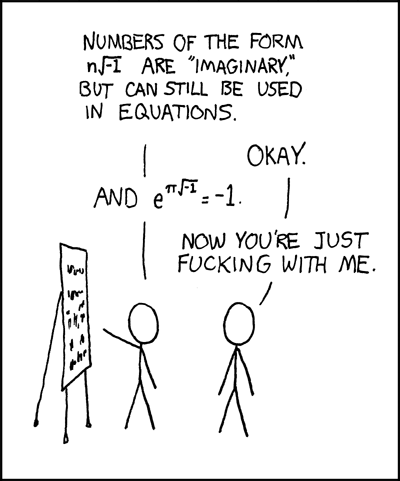
\includegraphics[width=0.33\textwidth]{pictures/etotheipi}
  \end{center}
%\caption{Positive Attitude}
\vspace{-20pt}
\caption{Die sch\"onste Formel der Welt!}
\end{wrapfigure}
In diesem Abschnitt lernen Sie eine zweite Darstellungsform f\"ur komplexe Zahlen kennen. Mit Hilfe dieser neuen Darstellungsform erhalten auch die Multiplikation und Division eine geometrische Bedeutung. Dies erm\"oglicht eine elegante Beschreibung von geometrischen Abbildungen und erleichtert die Potenzierung wesentlich.

Wie wir gesehen haben, lässt sich jede komplexe Zahl $z$ in der Gauss'schen Zahlenebene als Vektor darstellen. Dieser Vektor ist durch die Angabe des Real- und des Imaginärteils der komplexen Zahl $z$ eindeutig festgelegt.
Ein solcher vom Nullpunkt ausgehender Vektor lässt sich aber auch als Zeiger auffassen. Dieser Zeiger ist eindeutig festgelegt durch die Zeigerlänge $r$ und den Winkel $\varphi$, den der Zeiger mit der positiven reellen Achse einschliesst.
Als Beispiel betrachten wir den Zeiger mit der Länge $r = 2$ und dem Winkel $\varphi=45^\circ$.
\begin{center}
\definecolor{qqwuqq}{rgb}{0,0.39,0}
\definecolor{qqqqff}{rgb}{0,0,1}
\scalebox{1.2}{
\begin{tikzpicture}[line cap=round,line join=round,>=triangle 45,x=1.0cm,y=1.0cm]
\draw[->,color=black] (-2.72,0) -- (3.15,0);
\foreach \x in {-2,2}
\draw[shift={(\x,0)},color=black] (0pt,2pt) -- (0pt,-2pt) node[below] {\footnotesize $\x$};
\draw[color=black] (2.66,0.13) node [anchor=south west] {$\re$};
\draw[->,color=black] (0,-2.92) -- (0,3.22);
\foreach \y in {-2,2}
\draw[shift={(0,\y)},color=black] (2pt,0pt) -- (-2pt,0pt) node[left] {\footnotesize $\y \mathrm{i}$};
\draw[color=black] (0.14,2.58) node [anchor=west] {$\im$};
%\draw[color=black] (0pt,-10pt) node[right] {\footnotesize $0$};
\clip(-2.72,-2.92) rectangle (3.15,3.22);
\draw [shift={(0,0)},color=qqwuqq] (0,0) -- (0:0.8) arc (0:44.7:0.8) -- cycle;
\draw [->] (0,0) -- (1.42,1.4);
\draw [shift={(0,0)},->,color=qqwuqq] (0:0.8) arc (0:44.7:0.8);
\draw [dash pattern=on 4pt off 4pt] (0,0) circle (1cm);
\begin{scriptsize}
\fill [color=qqqqff] (1.42,1.4) circle (1.5pt);
\draw[color=qqqqff] (1.55,1.55) node {$z$};
\draw[color=qqwuqq] (0.5,0.2) node {$\varphi$};
\end{scriptsize}
\end{tikzpicture}
}
\end{center}
Dieser Zeiger besitzt 2-mal die Länge des zugeh\"origen Einheitszeigers. Er hat die Länge $1$ und schliesst mit der positiven reellen Achse den gleichen Winkel wie $z$ ein, also in unserem Beispiel $\varphi=45^\circ$.
F\"ur die komplexe Zahl $z$, die dem Zeiger mit der Länge $r = 2$ und dem Winkel $\varphi=45^\circ$ entspricht, schreiben wir
$$z=2\cdot \mathrm{e}^{\mathrm{i} 45^\circ}.$$
$\mathrm{e}^{\mathrm{i} 45^\circ}$ ist im Moment noch als reine Schreibweise aufzufassen. Erst später werden wir diesen Ausdruck beleuchten. Positive Winkel werden im Gegenuhrzeigersinn gemessen, negative Winkel im Uhrzeigersinn. Es ist dabei \"ublich, die Winkel im Bogenmass anzugeben. Im obigen Beispiel gilt dann
$$z=2\cdot \mathrm{e}^{\mathrm{i} 45^\circ}=2\cdot \mathrm{e}^{\mathrm{i} \frac{\pi}{4}}=\sqrt{2}+\mathrm{i}\sqrt{2}.$$

\begin{ueb}[Pythagoras]
Pr\"ufe das letzte Gleichheitszeichen mit einer Skizze und dem Satz von Pythagoras.
\end{ueb}

\begin{ueb}[Zeige, dass\dots]
Zeichne jeweils den entsprechenden Zeiger in eine Gauss'\-sche Zahlenebene ein. Notiere die Zahl auch in Normalform.\\[0ex]

(a) $z_1=3\cdot \mathrm{e}^{\mathrm{i}\pi}\q$ (b) $z_2=2\cdot \mathrm{e}^{\mathrm{i}\frac{3\pi}{2}}\q$ (c) $z_3=2\cdot \mathrm{e}^{-\mathrm{i}\frac{\pi}{2}}\q$ (d) $z_4=3\cdot \mathrm{e}^{\mathrm{i}3\pi}\q$ (e) $z_5=1\cdot \mathrm{e}^{\mathrm{i}\cdot 0}$
\end{ueb}

\begin{cdef}[Polarform]{def:polar}
Es sei $z\neq0$ eine komplexe Zahl. $z$ wird eindeutig durch die L\"ange $r=\abs{z}$ des zugeh\"origen Vektors und den Winkel $\varphi$, den der Vektor mit der positiven reellen Achse einschliesst, beschrieben. Man schreibt $z=r\mathrm{e}^{\mathrm{i}\varphi}$ und bezeichnet dies als die \emph{Polarform} von $z$. Der Winkel $\varphi$ zwischen $0$ und $2\pi$ wird als \emph{Argument} von $z$ bezeichnet. Man schreibt $\varphi=\arg{(z)}$.
\end{cdef}

\begin{bem}
$\varphi$ und $\varphi +k\cdot2\pi$ ($k\in\mZ$) ergeben stets dieselbe komplexe Zahl $z=r\mathrm{e}^{\mathrm{i}\varphi}$. In der Regel verwenden wir f\"ur $\varphi$ Winkelwerte zwischen $0$ und $2\pi$. Jedoch ist es manchmal zweckm\"assig, mit negativen Winkelwerten zu rechnen.
\end{bem}

\begin{ueb}[polar]
Gib folgende Zahlen in Polarform an: $3,3\mathrm{i},-3,-3\mathrm{i}$.
\end{ueb}

\begin{ueb}[Argument]
Es sei $z=4\cdot \mathrm{e}^{\mathrm{i}\frac{4\pi}{3}}$. Bestimme $\abs{z}, \arg{(z)}, \arg{(-z)}, \arg{(\bar{z})}$.
\end{ueb}

\begin{ueb}[Pfeilchen]
Zeichne die komplexen Zahlen
$$z_n=1\cdot \mathrm{e}^{\mathrm{i}\cdot n\frac{\pi}{3}}$$
f\"ur $n=0,1,2,\dots,5$ in eine Gauss'sche Zahlenebene ein. Was f\"ur eine Figur bilden die Punkte $z_0,\dots, z_5$.
\end{ueb}

Bei der Bearbeitung der letzten Aufgaben hat sich die Frage aufgedrängt: Wie bestimmt man in weniger einfachen F\"allen aus der Polarform $z = r\mathrm{e}^{\mathrm{i}\varphi}$ die Normalform $z = a + b\mathrm{i}$? Die Antwort ergibt sich mit Hilfe trigonometrischer Funktionen.

\begin{ueb}[Basics]
Leite die Formeln f\"ur $a$ und $b$ her, wenn die Polarform $z=r\cdot \mathrm{e}^{\mathrm{i}\varphi}$ bekannt ist.
\end{ueb}
Es gilt also
$$z=r\mathrm{e}^{\mathrm{i}\varphi}=r\cos(\varphi)+\mathrm{i}r\sin(\varphi)=a+b\mathrm{i}.$$
\begin{bem}
Da $re^{\mathrm{i}\varphi} = r (\cos(\varphi) + \mathrm{i}\sin(\varphi))$ ist, k\"onnen wir daraus ablesen, dass
$$e^{\mathrm{i}\varphi} = \cos(\varphi) + \mathrm{i}\sin(\varphi)$$
gelten muss. Diese Formel verkn\"upft die Exponentialfunktion, den Cosinus, den Sinus und die imaginäre Einheit $\mathrm{i}$ auf ganz \"uberraschende Weise.
In der Literatur wird daf\"ur oft der Ausdruck
$$\cis(\varphi)$$
anstelle von $\mathrm{e}^{\mathrm{i}\varphi}$ verwendet.
\end{bem}

\begin{bsp}
Wir betrachten $z=4\mathrm{e}^{\mathrm{i}\frac{3\pi}{4}}$. Es ist $r=4$ und $\varphi=\frac{3\pi}{4}$ und damit
$$z=4(\cos(\tfrac{3\pi}{4})+\mathrm{i}\sin(\tfrac{3\pi}{4}))=-2\sqrt{2}+\mathrm{i}2\sqrt{2}.$$
\end{bsp}

\begin{bem}
Da der Cosinus und der Sinus $2\pi$-periodisch sind (d.h. $\cos(\varphi + k \cdot 2\pi) = \cos(\varphi)$ sowie $\sin(\varphi + k \cdot 2\pi) = \sin(\varphi)$ f\"ur alle $k \in \mZ$), ist die obige Formel auch f\"ur negative Winkel oder solche gr\"osser als $2\pi$ richtig.
\end{bem}

\begin{ueb}[Normalform]
Berechne die Normalform der Zahlen

\begin{minipage}{0.3\textwidth}
\begin{enumeratea}
\item $1\cdot \mathrm{e}^\mathrm{i}$
\item $6\mathrm{e}^{\mathrm{i}\frac{5\pi}{3}}$
\end{enumeratea}
\end{minipage}
\begin{minipage}{0.4\textwidth}
\begin{enumeratea}
\setcounter{enumi}{2}
\item $\overline{\sqrt{2}\mathrm{e}^{\mathrm{i}\frac{5\pi}{4}}}$
\item $3\mathrm{e}^{\mathrm{i}\frac{\pi}{6}}-\sqrt{3}\mathrm{e}^{\mathrm{i}\frac{4\pi}{3}}$
\end{enumeratea}
\end{minipage}
\end{ueb}
Wir wissen nun also, wie man aus der Polarform einer komplexen Zahl die Normalform bestimmen kann. Wie aber geht man umgekehrt vor? Wie erhält man aus der Normalform $z = a + b\mathrm{i}$ die Polarform $z = r\mathrm{e}^{\mathrm{i}\varphi}$?

\begin{ueb}[Basics once again]
Leite zu $z = \sqrt{3} + \mathrm{i}$ die Polardarstellung her. Zeichne.
\end{ueb}

\begin{bem}
Bei der Berechnung der Polarform aus der Normalform muss man etwas vorsichtig sein. Zur Veranschaulichung berechnen wir die Polarform zu $w=-\sqrt{3}-\mathrm{i}$. Es ist zwar wiederum $r=\abs{z}=2$ und
$$\tan(\varphi)=\frac{-1}{-\sqrt{3}}=\frac{1}{\sqrt{3}},$$
was erneut zu $\varphi=\frac{\pi}{6}$ f\"uhrt. Ein Blick auf die Vektordarstellung von $w$ zeigt aber, dass $w$ im dritten Quadranten liegt und der zugeh\"orige Winkel daher $\tilde{\varphi}=\varphi+\pi=\frac{7\pi}{6}$ beträgt.
\begin{center}
\definecolor{qqwuqq}{rgb}{0,0.39,0}
\scalebox{0.95}{
\begin{tikzpicture}[line cap=round,line join=round,>=triangle 45,x=1.7cm,y=1.7cm]
\draw[->,color=black] (-2.07,0) -- (2.07,0);
\foreach \x in {-2,-1,1,2}
\draw[shift={(\x,0)},color=black] (0pt,2pt) -- (0pt,-2pt);
\draw[color=black] (1.98,0.02) node [anchor=south west] {$\mR$};
\draw[->,color=black] (0,-1.51) -- (0,1.48);
\foreach \y in {-1,1}
\draw[shift={(0,\y)},color=black] (2pt,0pt) -- (-2pt,0pt);
\draw[color=black] (0.03,1.36) node [anchor=west] {$\mathrm{i}\mR$};
\clip(-2.07,-1.51) rectangle (2.07,1.48);
\draw [shift={(0,0)},color=qqwuqq,fill=qqwuqq,fill opacity=0.1] (0,0) -- (0:0.42) arc (0:30.03:0.42) -- cycle;
\draw [shift={(0,0)},color=qqwuqq,fill=qqwuqq,fill opacity=0.1] (0,0) -- (180:0.42) arc (180:210.03:0.42) -- cycle;
\draw [shift={(1.73,0)},color=qqwuqq,fill=qqwuqq,fill opacity=0.1] (0,0) -- (90.07:0.16) arc (90.07:180:0.16) -- cycle;
\draw [shift={(0,0)},color=qqwuqq] (0,0) -- (0:0.21) arc (0:180:0.21) -- cycle;
\draw [->] (0,0) -- (1.73,1);
\draw [->] (0,0) -- (-1.73,-1);
\draw [dash pattern=on 1pt off 1pt] (-1.73,-1)-- (-1.73,0);
\draw [dash pattern=on 1pt off 1pt] (-1.73,-1)-- (0,-1);
\draw [dash pattern=on 1pt off 1pt] (0,1)-- (1.73,1);
\draw [dash pattern=on 1pt off 1pt] (1.73,1)-- (1.73,0);
\draw [shift={(0,0)},->,color=qqwuqq] (0:0.42) arc (0:30.03:0.42);
\draw [shift={(0,0)},->,color=qqwuqq] (180:0.42) arc (180:210.03:0.42);
\draw [shift={(0,0)},->,color=qqwuqq] (0:0.21) arc (0:180:0.21);
\begin{scriptsize}
\fill [color=black] (1.73,1) circle (1.5pt);
\draw[color=black] (1.77,1.2) node {$z$};
\fill [color=black] (-1.73,-1) circle (1.5pt);
\draw[color=black] (-1.9,-1) node {$w$};
%\fill [color=black] (-1.73,0) circle (1.5pt);
\draw[color=black] (-1.69,0.15) node {$-\sqrt{3}$};
%\fill [color=black] (0,-1) circle (1.5pt);
\draw[color=black] (0.2,-1) node {$-\mathrm{i}$};
%\fill [color=black] (0,1) circle (1.5pt);
\draw[color=black] (-0.1,1.07) node {$\mathrm{i}$};
%\fill [color=black] (1.73,0) circle (1.5pt);
\draw[color=black] (1.77,-0.2) node {$\sqrt{3}$};
\draw[color=qqwuqq] (0.28,0.08) node {$\varphi$};
\draw[color=qqwuqq] (-0.28,-0.08) node {$\varphi$};
\draw[color=qqwuqq] (1.67,0.08) node {$\cdot$};
\draw[color=qqwuqq] (-0.1,0.3) node {$\pi$};
\end{scriptsize}
\end{tikzpicture}
}
\end{center}
Wir m\"ussen also zum Winkel $\varphi$ noch $\pi$ addieren, um in den richtigen Quadranten zu gelangen. Die Mehrdeutigkeit kommt daher zustande, dass der Tangens $\pi$-periodisch ist.
\end{bem}

\begin{csatz}{Polar- und Normalform}{satz:polnorm}
Es sei $z\in\mC$. Ist $z=r\mathrm{e}^{\mathrm{i}\varphi}$ mit $r>0$ und $\varphi\in\mR$ in Polarform gegeben, dann ist die Normalform
$$z=r(\cos(\varphi)+\mathrm{i}\sin(\varphi))=r\cos(\varphi)+\mathrm{i}r\sin(\varphi)).$$

Ist $z=a+b\mathrm{i}$ in Normalform gegeben, dann ist in der Polarform
$$r=\abs{z}=\sqrt{a^2+b^2}$$
und
$$\varphi=\tan^{-1}(\tfrac{b}{a}),$$
bis auf ein additives $\pi$.
\end{csatz}

\begin{ueb}[Polarform]
Berechne die Polarform der Zahlen\\

(a) $1+\mathrm{i}\q$ (b) $-5+3\mathrm{i}\q$ (c) $-1-\sqrt{3}\mathrm{i}\q$ (d) $\sqrt{7}-\frac{1}{2}\mathrm{i}$
\end{ueb}

\begin{ueb}[und nochmal]
Es sei $z=2+4\mathrm{i}$ und $w=-1+2\mathrm{i}$. Berechne\\

(a) $\arg{(z\cdot w)}\q$ (b) $\abs{\frac{z}{w-3\mathrm{i}}}\q$ (c) die Polarform von $\frac{w}{z}$
\end{ueb}

\clearpage

\section{Die Multiplikation und Division in Polarform}

Die Addition und Subtraktion zweier komplexer Zahlen k\"onnen wir geometrisch als Vektoraddition, bzw. -subtraktion ihrer zugeh\"origen Vektoren interpretieren. Mit Hilfe der Polarform lässt sich nun auch die Multiplikation, bzw. Division zweier komplexer Zahlen geometrisch deuten.

\begin{ueb}[Multiplikation polar]
Es sei $z_1=\frac{2}{3}+\frac{3\sqrt{3}}{2}\mathrm{i}$ und $z_2=\sqrt{3}+\mathrm{i}$.
\begin{enumeratea}
\item Berechne das Produkt $z_1\cdot z_2$ in Polar- und Normalform.
\item Wie lautet die Vorschrift f\"ur die Multiplikation in Polarform?
\end{enumeratea}
\end{ueb}
\noindent Die obige Aufgabe lässt vermuten: Komplexe Zahlen werden multipliziert, indem man ihre Beträge multipliziert und ihre Argumente addiert. Um diese Vermutung zu bestätigen, betrachten wir nun die Multiplikation in allgemeiner Form.

\begin{ueb}[juhuu!]
Zeige die Vermutung mit $z_1=r_1\cis(\varphi_1)$ und $z_2=r_2\cis(\varphi_2)$.
\end{ueb}

\begin{csatz}[Multiplikation polar]{satz:mulpolar}
Sind $z_1=r_1\mathrm{e}^{\mathrm{i}\varphi_1}$ und $z_2=r_2\mathrm{e}^{\mathrm{i}\varphi_2}$ zwei komplexe Zahlen, dann gilt
$$z_1\cdot z_2=(r_1r_2)\cdot \mathrm{e}^{\mathrm{i}(\varphi_1+\varphi_2)}.$$
\end{csatz}

\begin{bem}
Diese Rechenvorschrift kann man sich leicht merken, wenn man $\mathrm{e}^{\mathrm{i}\varphi}$ als \glqq $\mathrm{e}$ hoch $\mathrm{i}$ mal $\varphi$\grqq\ interpretiert. F\"ur Potenzen mit gleicher Basis gilt nämlich nach dem Potenzgesetz: $\mathrm{e}^m\cdot \mathrm{e}^n = \mathrm{e}^{m+n}$.
\end{bem}

\begin{ueb}[Potenzieren]
Berechne folgende Ausdr\"ucke:\\

(a) $3\mathrm{e}^{\mathrm{i}\frac{\pi}{12}}\cdot 4\mathrm{e}^{\mathrm{i}\frac{\pi}{6}}\q$ (b) $\mathrm{e}^{\mathrm{i}\frac{\pi}{3}}\mathrm{e}^{\mathrm{i}\frac{2\pi}{3}}\mathrm{e}^{\mathrm{i}\pi}\mathrm{e}^{\mathrm{i}\frac{4\pi}{3}}\mathrm{e}^{\mathrm{i}\frac{5\pi}{3}}\q$ (c) $\left(2\mathrm{e}^{\mathrm{i}\frac{\pi}{4}}\right)^2$
\end{ueb}

\begin{ueb}[Moivre]
Es sei $z=r\mathrm{e}^{\mathrm{i}\varphi}$ eine komplexe Zahl und $n\in\mN$. Wie lautet die Polarform $z^n$?
\end{ueb}

\begin{ueb}[de Moivre]
Berechne $(1+\mathrm{i})^6+(1-\mathrm{i})^6$. Verwende einmal das Pascalsche Dreieck und gehe ein ander mal über die Polarform, um zu potenzieren.
\end{ueb}

\begin{ueb}[Einheit]
Es sei $z=r\mathrm{e}^{\mathrm{i}\varphi}\neq0$ eine komplexe Zahl. Mit welcher Zahl muss $z$ multipliziert werden, damit das Produkt $1$ ergibt.
\end{ueb}

\begin{bem}
F\"ur die $n$-te Potenz, bzw. f\"ur den Kehrwert einer komplexen Zahl $z=r\mathrm{e}^{\mathrm{i}\varphi}$ gilt:
$$z^n=\left(r\mathrm{e}^{\mathrm{i}\varphi}\right)^n=r^n\mathrm{e}^{\mathrm{i}n\varphi},$$
bzw.
$$\frac{1}{z}=z^{-1}=\left(re^{\mathrm{i}\varphi}\right)^{-1}=r^{-1}\mathrm{e}^{\mathrm{i}(-\varphi)}.$$
\end{bem}
\noindent Mit diesem Resultat lässt sich die Division zweier komplexer Zahlen trivialerweise auf die Multiplikation zur\"uckf\"uhren. Im Grunde genommen ist eine Divison ja eine Multiplikation mit dem enstprechenden inversen Element.

\begin{csatz}[Division polar]{satz:divpolar}
Sind $z_1=r_1\mathrm{e}^{\mathrm{i}\varphi_1}$ und $z_2=r_2\mathrm{e}^{\mathrm{i}\varphi_2}$ zwei komplexe Zahlen, dann gilt
$$\frac{z_1}{z_2}=\frac{r_1}{r_2}\cdot \mathrm{e}^{\mathrm{i}(\varphi_1-\varphi_2)}.$$
\end{csatz}

\begin{ueb}[Rechnen]
Berechne f\"ur $v=2\mathrm{e}^{\mathrm{i}\frac{5\pi}{6}}$, $w=3\mathrm{e}^{\mathrm{i}\frac{3\pi}{4}}$, $z=4\mathrm{e}^{\mathrm{i}\frac{\pi}{12}}$ die folgenden Ausdr\"ucke und gib das Ergebnis in Polarform an.\\

(a) $\frac{v\cdot w}{z}\q$ (b) $w^{-3}\q$ (c) $z^2\div v^5$
\end{ueb}

\begin{ueb}[beide Formen haben ihre Vor- und Nachteile]
Bestimme das Ergebnis des folgenden Ausdrucks in Polarform und in Normalform:
$$\frac{\mathrm{i}^{10}}{\left(\sqrt{3}-\mathrm{i}\right)^4}.$$
\end{ueb}

\begin{ueb}[Division einfach gemacht]
Zeige: Sind $z_1$ und $z_2\neq0$ komplexe Zahlen, so ist $\overline{z_1\div z_2}=\overline{z_1}\div\overline{z_2}$.
\end{ueb}

\clearpage

\section{Alle quadratischen Gleichungen sind l\"osbar!}

\begin{wrapfigure}{r}{0.382\textwidth}
\vspace{-22pt}
  \begin{center}
    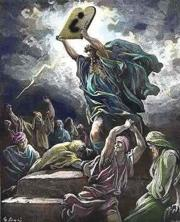
\includegraphics[width=0.38\textwidth]{pictures/imagin}
  \end{center}
\caption{Gleichungen sind l\"osbar}
\vspace{-22pt}
\end{wrapfigure}
In diesem Kapitel lernen Sie eine erste wichtige Anwendung der komplexen Zahlen kennen: Im Bereich der komplexen Zahlen sind \emph{alle} quadratischen Gleichungen l\"osbar!
Dies ist eine verbl\"uffende Tatsache. Wir haben mit der Definition von $\mathrm{i}$ die L\"osbarkeit einer quadratischen Gleichung gefordert, nämlich $x^2 = -1$. Nun zeigt sich, dass damit alle quadratischen Gleichungen l\"osbar sind. So ist das häufig in der Mathematik: Ein kleiner Schritt hat eine grosse Wirkung.
\begin{bem}
Effektiv sind nun sogar alle Polynomgleichungen $n$-ten Grades l\"osbar. Eine Entdeckung von, na wem wohl, \textsc{Carl Friedrich Gauss}.
\end{bem}

\subsection{Beispiele f\"ur quadratische Gleichungen mit komplexen L\"osungen}
Zu Beginn sind wir von der Gleichung
$$z^2 = -1$$
ausgegangen. Diese quadratische Gleichung ist in $\mR$ nicht l\"osbar --- wohl aber in $\mC$, wie Sie jetzt wissen. Sie besitzt die L\"osung $\mathrm{i}$. Wir schreiben f\"ur die Unbekannte nun $z$ statt $x$, um anzudeuten, dass wir auch L\"osungen in $\mC$ zulassen wollen. Offensichtlich ist aber auch
$$(-\mathrm{i})^2 = (-1)^2 \cdot \mathrm{i}^2 = 1 \cdot (-1) = -1.$$
Also ist $-\mathrm{i}$ ebenfalls eine L\"osung der Gleichung $z^2 = -1$. Insgesamt besitzt die quadratische Gleichung $z^2=-1$ zwei L\"osungen, nämlich
$$z_1=\mathrm{i}\text{ und }z_2=-\mathrm{i}.$$
\begin{bem}
Weitere L\"osungen sind nicht m\"oglich: $z^2 = -1$ ist äquivalent zu der Gleichung $z^2 - (-1) = 0$, und es gilt
$$0 = z^2 -(-1) = z^2 -\mathrm{i}^2 = (z-\mathrm{i})(z+\mathrm{i}),$$
wobei im letzten Schritt die dritte binomische Formel benutzt wurde. Ein Produkt ist aber genau dann null, wenn einer der beiden Faktoren null ist. Also gibt es nur die beiden L\"osungen $z_1 = \mathrm{i}$ und $z_2 = -\mathrm{i}$.
\end{bem}
Wie gehen wir nun bei der Gleichung
$$z^2 = -2$$
vor? Ganz einfach, wir schreiben $z^2 = 2 \cdot (-1)$ und finden die beiden konjugiert komplexen L\"osungen
$$z_1 = \sqrt{2}\mathrm{i}\text{ und }z_2=-\sqrt{2}\mathrm{i}.$$

\begin{ueb}[QuadrGL komplex]
Gib alle L\"osungen der folgenden Gleichungen an.

\begin{minipage}{3.5cm}
\begin{enumeratea}
\item $z^2=-4$
\item $z^2+3=0$
\end{enumeratea}
\end{minipage}
\begin{minipage}{3.5cm}
\begin{enumeratea}
\setcounter{enumi}{2}
\item $6z^2=15$
\item $z^3=-8z$
\end{enumeratea}
\end{minipage}
\end{ueb}

\subsection{Quadratisches Ergänzen}
Im vorigen Abschnitt haben wir quadratische Gleichungen betrachtet, in denen $z$ nur als $z^2$ vorkam. Wir konnten sie leicht l\"osen, indem wir sie auf die Form $(\dots)^2 = \text{Zahl}$ gebracht haben.
Im Allgemeinen ist eine quadratische Gleichung aber von der Form
$$az^2+bz+c = 0$$
mit $a, b, c$ reell und $a\neq 0$. Wie lässt sich eine solche Gleichung l\"osen?
Als Beispiel sehen wir uns die folgende quadratische Gleichung an:
$$z^2 -6z+13=0.$$
Lässt sich diese Gleichung auch auf die soeben behandelte Form $(\dots)^2 = \text{Zahl}$ bringen? Denn dann k\"onnen wir versuchen, unsere L\"osungsmethode aus dem vorigen Abschnitt auf diese Gleichung anzuwenden.
Um die linke Seite der Gleichung als Quadrat zu schreiben, benutzen wir die Methode des quadratischen Ergänzens. In unserem Beispiel funktioniert dies wie folgt:
$$
0=z^2-6z+13=[z^2-6z]+13=[(z-3)^2-9]+13=(z-3)^2+4
$$
Die Gleichung $z^2-6z+13 = 0$ ist somit äquivalent zur Gleichung $(z-3)^2+4 = 0$. Auf den ersten Blick sieht die umgeformte Gleichung viel komplizierter aus als zuvor, aber bei näherer Betrachtung lässt sie sich wie die im vorigen Abschnitt behandelten Gleichungen l\"osen.
\begin{ueb}[ergänzt]
Bestimme alle L\"osungen von
$$z^2-6z+13 = 0.$$
\end{ueb}
\noindent Die Gleichung $z^2 - 6z + 13 = 0$ besitzt also die beiden L\"osungen
$$z_1 =3+2\mathrm{i}\text{ und }z_2 =3-2\mathrm{i}.$$

\subsection{Die allgemeine L\"osungsformel f\"ur quadratische Gleichungen}

Die allgemeine quadratische Gleichung ist von der Form
$$az^2+bz+c=0$$
mit $a,b,c\in\mR$ und $a\neq0$.

\begin{ueb}[Repe]
Leite die L\"osungsformel f\"ur quadratische Gleichungen her. Tipp: Benutze quadratische Ergänzung.
\end{ueb}

\begin{ueb}[zauberformelhaft]
Finde alle L\"osungen der Gleichung
$$z^2+\frac{1}{2}z+3=0.$$
\end{ueb}

\begin{ueb}[erweitere QuadrGL]
Finde alle L\"osungen der folgenden Gleichungen\\[0ex]

(a) $z^2-4z+20=0\q$ (b) $\frac{4}{5}z-\frac{1}{5}z^2=-9\q$ (c) $2z^2-z+1=0$
\end{ueb}

\begin{ueb}[netter Zusammenhang]
Zeige: Ist
$$az^2+bz+c=0$$
eine quadratische Gleichung mit $a,b,c\in\mR$, dann ist das Produkt der L\"osungen reell.
\end{ueb}

\begin{ueb}[umgekehrt]
Die Gleichung
$$z^2-2z+a=0$$
mit $a\in\mR$ habe die L\"osung $z_1=1+\mathrm{i}.$ Bestimme $a$ und die zweite L\"osung $z_2$.
\end{ueb}

\begin{bem}
Die obige L\"osungsformel gilt nach dem Permanenzprinzip auch f\"ur quadratische Gleichungen mit komplexen Koeffizienten, d.h. f\"ur Gleichungen $az^2 + b^z + c = 0$ mit $a, b, c$ komplex.
\end{bem}

\begin{ueb}[und komplex]
Findest du die L\"osungen von
$$z^2-z+\frac{1}{4}-\frac{1}{2}\mathrm{i}=0?$$
\end{ueb}

\begin{ueb}[und nochmal komplex]
Löse die Gleichung
$$z^2+\mathrm{i}z=4z-5-\mathrm{i}$$
\end{ueb}

\newpage

\appendix

\section{Historisches und Impact}
\begin{wrapfigure}{r}{0.382\textwidth}
\vspace{-15pt}
  \begin{center}
    
\includegraphics[width=0.38\textwidth]{pictures/doiexist}
  \end{center}
\caption{\glqq Do I really Exist?\grqq}
\end{wrapfigure}
Um 1530 st\"osst eine Gruppe italienischer Mathematiker beim L\"osen von Gleichungen auf unbekannte Zahlen, die nicht f\"urs Zählen oder Messen von Dingen gebraucht werden k\"onnen.
\marginnote{
\qrcode{
https://youtu.be/nT3vgrauJ8A}
}
Die Zahlen schienen nutz- und sinnlos. Der franz\"osische Philosoph \textsc{René Descartes} teilte die damals gängige Meinung der Mathematiker und gab diesen Zahlen einen Namen: imaginäre Zahlen.

Nach langem Widerstand wurden im 19.-ten Jahrhundert die imaginären Zahlen akzeptiert und bald darauf entdeckte man ihre N\"utzlichkeit. Heute sind imagin\"are Zahlen aus der Mathematik und Technik nicht mehr wegzudenken. Ohne imagin\"are Zahlen gäbe es Radio/Fernsehen in der heutigen Form nicht. Auch die digitale Fotographie oder das Internet w\"aren nicht realisierbar. Ferner lieferten die imagin\"aren Zahlen enorme Fortschritte in der Insulinforschung, Virenforschung oder DNA-Analyse. Alle Wissenschaften, die auf komplexe, umfangreiche Simulationen angewiesen sind --- z.B. Meteorologie, Geologie, Klimatologie, \dots --- sind auf imaginäre Zahlen angewiesen.

\section{Punktmengen in der Gauss'schen Zahlenebene}

\begin{ueb}[Abstände]
Zeichne in der Gauss'schen Zahlenebene und markiere in verschiedenen Farben die Menge aller Punkte $z$ mit

\begin{minipage}{3.5cm}
\begin{enumeratea}
\item $\abs{z}=1$
\item $\abs{z+1}=1$
\end{enumeratea}
\end{minipage}
\begin{minipage}{3.5cm}
\begin{enumeratea}
\setcounter{enumi}{2}
\item $\abs{z-(1+\mathrm{i})}=1$
\item $\abs{z-1}=\abs{z-3}$
\end{enumeratea}
\end{minipage}
\end{ueb}

\begin{bem}
F\"ur eine komplexe Zahl $z$ ist die Gleichung
$$\abs{z-m}=r$$
mit $m$ komplex und $r$ positiv ein Kreis mit Mittelpunkt $m$ und Radius $r$ in der Gauss'\-schen Zahlenebene.
\end{bem}

Beispielsweise kann die Einheitskreisscheibe, inklusive Rand, durch
$$\abs{z}\leq 1$$
dargestellt werden. Oder die Menge aller Punkte in der Gauss'\-schen Zahlenebene ohne die Kreisscheibe mit Radius $2$ um $\point{-1}{0}$ ist gegeben durch
$$\abs{z+1}>2.$$
Bei diesen einfachen Beispielen kann man intuitiv erkennen, wie die Punktmenge aussieht. Wie findet man die Punktmenge bei nichttrivialen Bedingungen?

\begin{bsp}
Wir bestimmen rechnerisch, welche Punktmenge durch die Gleichung
$$\abs{\frac{z-3}{z+1}}\geq1$$
bestimmt ist. Das k\"onnen wir mit verschiedenen †berlegungen erreichen.

\begin{description}
\item[1. Methode] Man rechnet die Beträge aus
\begin{align*}
\abs{\frac{z-3}{z+1}}&\geq1\\
\abs{z-3}&\geq\abs{z+1}\\
\sqrt{(a-3)^2+b^2}&\geq\sqrt{(a+1)^2+b^2}\\
a^2-6a+9+b^2&\geq a^2+2a+1+b^2\\
8&\geq 8a\\
a&\leq1
\end{align*}
D.h. die L\"osung sind alle Punkte in der Halbebene $a\leq1$ ohne $z=-1$.
\item[2. Methode] Man benutzt die Beziehung $\abs{z}^2=z\cdot\bar{z}$, woraus
\begin{align*}
\abs{\frac{z-3}{z+1}}^2&\geq1\\
\frac{(z-3)(\bar{z}-3)}{(z+1)(\bar{z}+1)}&\geq1\\
z\bar{z}-3z-3\bar{z}+9&\geq z\bar{z}+z+\bar{z}+1\\
8&\geq 4(z+\bar{z})=8a\\
a&\leq1
\end{align*}
\item[3. Methode] Man \"uberlegt sich, was die Ungleichung geometrisch bedeutet. Hier sind alle Zahlen $z$ gesucht, f\"ur die der Abstand von $3$ gr\"osser oder gleich dem Abstand von $-1$ ist. Diese Punkte liegen offensichtlich in der Halbebene $a\leq1$.
\end{description}
\end{bsp}

\begin{ueb}[Apollonios-Kreis]
Zeichne die Menge aller Punkte
$$\abs{\frac{z-5}{z+1}}\geq2,$$
einen sogenannten \emph{Apollonios-Kreis}\footnote{In der Geometrie ist der \textbf{Kreis des Apollonios} ein spezieller geometrischer Ort, nämlich die Menge aller Punkte, f\"ur die das Verhältnis der Entfernungen zu zwei vorgegebenen Punkten einen vorgegebenen Wert hat.}
\end{ueb}

Wir schreiben allgemein f\"ur den Kreis
\marginnote{
\qrcode{
https://www.youtube.com/watch?v=yDTCIyukwBg}
}
$k$ mit Mittelpunkt $M\in\mathbb{C}$ und Radius $r\in\mR$
$$k(M,r)=\setm{z\in\mathbb{C}}{\abs{z-M}=r},$$
wobei $r\in\mR$.

Aus der Betragsfunktion erkennen wir die \emph{Kreisgleichung}, denn aus $\abs{z-M}^2=r^2$ folgt die Form
$$z\bar{z}-M\bar{z}-\bar{M}z+s=0.$$
Ohne den Produktterm $z\bar{z}$ stellt
$$p\bar{z}+\bar{p}z+s=0$$
eine \emph{Gerade} dar:
$$y=-\frac{a}{b}x-\frac{s}{2b}.$$

\begin{ueb}[Kehrwert]
Zeige:
$$\abs{z}=1\implies\bar{z}=\frac{1}{z}.$$
\end{ueb}

\begin{ueb}[Punktmengen]
Bestimme die Punktmenge gegeben durch die Gleichungen

\begin{minipage}{0.3\textwidth}
\begin{enumeratea}
\item $\abs{z-1+\mathrm{i}}<2$
\item $\abs{\frac{z+\mathrm{i}}{z-3\mathrm{i}}}\leq1$
\end{enumeratea}
\end{minipage}
\begin{minipage}{0.4\textwidth}
\begin{enumeratea}
\setcounter{enumi}{2}
\item $\abs{\frac{z-2}{z+2\mathrm{i}}}=1$
\item $\abs{\frac{z-5\mathrm{i}}{z+\mathrm{i}}}\geq2$
\end{enumeratea}
\end{minipage}
\end{ueb}

\begin{ueb}[Kreis]
Stellt die Gleichung
$$z\bar{z}-(3-\mathrm{i})\bar{z}-(3+\mathrm{i})z-6=0$$
einen Kreis dar? Falls ja, bestimme Mittelpunkt und Radius.
\end{ueb}

\begin{ueb}[Geraden]
Welche Punktmenge wird durch
$$\abs{z-1}+\abs{z+1}=4$$
dargestellt?
\end{ueb}

\section{e hoch i mal phi}

Wir haben f\"ur die Polarform einer komplexen Zahl die Schreibweise $r\mathrm{e}^{\mathrm{i}\varphi}$ (\glqq $r$-mal Einheitszeiger mit Winkel $\varphi$\grqq) eingef\"uhrt. Dabei handelte es sich bis jetzt um eine reine Schreibweise. Von der Interpretation \glqq $\mathrm{e}$ hoch $\mathrm{i}$ mal $\varphi$\grqq\ haben wir bei allen Herleitungen oder Beweisen keinen Gebrauch gemacht. In diesem Abschnitt werden wir plausibel machen, dass die komplexe Zahl $\mathrm{e}^{\mathrm{i}\varphi}$ tatsächlich als $\mathrm{e}$ hoch $\mathrm{i}$ mal $\varphi$ zu verstehen ist.
Die Zahl
$$\mathrm{e} = 2.718281828459\dots$$
wurde nach dem Schweizer Mathematiker und Physiker \textsc{Leonhard Euler} (1707-1783) benannt. Diese sogenannte \textbf{Eulersche Zahl} $\mathrm{e}$ ist definiert als
$$\mathrm{e}:=\lim_{n\to\infty}\left(1+\frac{1}{n}\right)^n$$
Dies wird durch Tabelle \ref{tab:e} auf Seite \pageref{tab:e} verdeutlicht. Die Zahlen $(1+\frac{1}{n})^n$ nähern sich f\"ur $n$ gegen unendlich immer mehr und ausschliesslich der bestimmten Zahl $2.718\dots.$
\begin{table}
\begin{center}
\begin{tabular}{|c|l|}
\hline
\rowcolor{lightyellow}\spaltenheight    $n$ & $(1+\frac{1}{n})^n$\spaltensep\hline\hline
\rowcolor{Gray}\spaltenheight 1 & 2\spaltensep\hline
\rowcolor{lightyellow}\spaltenheight    2 & 2.25\spaltensep\hline
\rowcolor{Gray}\spaltenheight 10 & 2.59\dots\spaltensep\hline
\rowcolor{lightyellow}\spaltenheight    100 & 2.70\dots\spaltensep\hline
\rowcolor{Gray}\spaltenheight 1000 & 2.716\dots\spaltensep\hline
\rowcolor{lightyellow}\spaltenheight    100000 & 2.71826\dots\spaltensep\hline
\rowcolor{Gray}\spaltenheight 100000000 & 2.71828\dots\spaltensep\hline
\end{tabular}
\end{center}
\caption{Approximation an $\mathrm{e}$}\label{tab:e}
\end{table}
Allgemeiner gilt f\"ur jede Zahl $a\in\mR$
$$\mathrm{e}^a=\lim_{n\to\infty}\left(1+\frac{a}{n}\right)^n,$$
was im Spezialfall $a=1$ mit dem Obigen \"ubereinstimmt. In diesem Ausdruck treten nur Grundrechenoperationen auf, die auch in $\mC$ ausgef\"uhrt werden k\"onnen. Wegen des Permanenzprinzips sollte also auch $\mathrm{e}^z$ mit $z\in\mC$ definiert sein.

\begin{bsp}
Wir versuchen
$$\lim_{n\to\infty}\left(1+\frac{\mathrm{i}}{n}\cdot\frac{\pi}{2}\right)^n$$
zu bestimmen. Wir betrachten die Entwicklung in Tabelle \ref{tab:exp} auf Seite \pageref{tab:exp}.

\begin{table}
\begin{center}
\begin{tabular}{|c|c|}
\hline
\rowcolor{lightyellow}\spaltenheight    $n$ & $(1+\frac{\mathrm{i}}{n}\cdot\frac{\pi}{2})^n$\spaltensep\hline\hline
\rowcolor{Gray}\spaltenheight 1 & $1+\mathrm{i}\cdot 1.570796\dots$\spaltensep\hline
\rowcolor{lightyellow}\spaltenheight    2 & $0.383149\dots+i\cdot 1.570796\dots$\spaltensep\hline
\rowcolor{Gray}\spaltenheight 10 & $0.014381\dots+\mathrm{i}\cdot 1.129518\dots$\spaltensep\hline
\rowcolor{lightyellow}\spaltenheight    100 & $0.000130\dots+\mathrm{i}\cdot 1.012411\dots$\spaltensep\hline
\rowcolor{Gray}\spaltenheight 1000 & $0.000001\dots+\mathrm{i}\cdot 1.001234\dots$\spaltensep\hline
\rowcolor{lightyellow}\spaltenheight    100000 & $0.000000\dots+i\cdot 1.000012\dots$\spaltensep\hline
\end{tabular}
\end{center}
\caption{Approximation an $\mathrm{e}^{\mathrm{i}\frac{\pi}{2}}$}\label{tab:exp}
\end{table}
\noindent Geometrisch sehen die ersten drei Näherungen wie folgt aus:
\begin{center}
\definecolor{qqwuqq}{rgb}{0,0.39,0}
\definecolor{qqqqff}{rgb}{0,0,1}
\scalebox{1.5}{
\begin{tikzpicture}[line cap=round,line join=round,>=triangle 45,x=1.2cm,y=1.2cm]
\draw[->,color=black] (-0.37,0) -- (1.3,0);
\foreach \x in {0.5,1}
\draw[shift={(\x,0)},color=black] (0pt,2pt) -- (0pt,-2pt) node[below] {\footnotesize $\x$};
\draw[color=black] (1.15,0.04) node [anchor=south west] {$\mR$};
\draw[->,color=black] (0,-0.37) -- (0,1.98);
\foreach \y in {0.5,1,1.5}
\draw[shift={(0,\y)},color=black] (2pt,0pt) -- (-2pt,0pt) node[left] {\footnotesize $\y$};
\draw[color=black] (0.04,1.79) node [anchor=west] {$\mathrm{i}\mR$};
%\draw[color=black] (0pt,-10pt) node[right] {\footnotesize $0$};
\clip(-0.37,-0.37) rectangle (1.3,1.98);
\draw [shift={(0,0)},color=qqwuqq,fill=qqwuqq,fill opacity=0.1] (0,0) -- (0:0.43) arc (0:57.52:0.43) -- cycle;
\draw [->] (0,0) -- (1,1.57);
\begin{scriptsize}
\fill [color=qqqqff] (1,1.57) circle (1.5pt);
\draw[color=qqqqff] (0.95,1.69) node {$1+i\frac{\pi}{2}$};
\draw[color=qqwuqq] (0.28,0.13) node {$\varphi_1$};
\end{scriptsize}
\end{tikzpicture}
}
\definecolor{qqwuqq}{rgb}{0,0.39,0}
\definecolor{qqqqff}{rgb}{0,0,1}
\scalebox{1.5}{
\begin{tikzpicture}[line cap=round,line join=round,>=triangle 45,x=1.25cm,y=1.25cm]
\draw[->,color=black] (-0.31,0) -- (1.46,0);
\foreach \x in {,0.5,1}
\draw[shift={(\x,0)},color=black] (0pt,2pt) -- (0pt,-2pt) node[below] {\footnotesize $\x$};
\draw[color=black] (1.35,0.03) node [anchor=south west] {$\mR$};
\draw[->,color=black] (0,-0.3) -- (0,1.87);
\foreach \y in {,0.5,1,1.5}
\draw[shift={(0,\y)},color=black] (2pt,0pt) -- (-2pt,0pt) node[left] {\footnotesize $\y$};
\draw[color=black] (0.03,1.74) node [anchor=west] {$\mathrm{i}\mR$};
%\draw[color=black] (0pt,-10pt) node[right] {\footnotesize $0$};
\clip(-0.31,-0.3) rectangle (1.46,1.87);
\draw [shift={(0,0)},color=qqwuqq,fill=qqwuqq,fill opacity=0.1] (0,0) -- (0:0.32) arc (0:38.15:0.32) -- cycle;
\draw [shift={(0,0)},color=qqwuqq,fill=qqwuqq,fill opacity=0.1] (0,0) -- (38.15:0.32) arc (38.15:76.29:0.32) -- cycle;
\draw [shift={(1,0.79)},color=qqwuqq,fill=qqwuqq,fill opacity=0.1] (0,0) -- (128.15:0.19) arc (128.15:218.15:0.19) -- cycle;
\draw [->] (0,0) -- (0.38,1.57);
\draw (0,0)-- (1,0.79);
\draw (0.38,1.57)-- (1,0.79);
\draw (1,0.79)-- (1,0);
\fill[color=qqwuqq,fill=qqwuqq,fill opacity=0.1] (0.89,0.8) circle (0.01);
\begin{scriptsize}
\fill [color=qqqqff] (0.38,1.57) circle (1.5pt);
%\draw[color=qqqqff] (0.43,1.65) node {$z$};
\fill [color=qqqqff] (1,0.79) circle (1.5pt);
\draw[color=qqqqff] (1,1) node {$1+\frac{\pi}{2}\frac{i}{2}$};
\draw[color=qqwuqq] (0.5,0.15) node {$\varphi_2$};
\draw[color=qqwuqq] (0.31,0.4) node {$\varphi_2$};
\end{scriptsize}
\end{tikzpicture}
}
\definecolor{qqwuqq}{rgb}{0,0.39,0}
\definecolor{qqqqff}{rgb}{0,0,1}
\scalebox{1.5}{
\begin{tikzpicture}[line cap=round,line join=round,>=triangle 45,x=1.3cm,y=1.3cm]
\draw[->,color=black] (-0.31,0) -- (1.38,0);
\foreach \x in {,0.5,1}
\draw[shift={(\x,0)},color=black] (0pt,2pt) -- (0pt,-2pt) node[below] {\footnotesize $\x$};
\draw[color=black] (1.27,0.03) node [anchor=south west] {$\mR$};
\draw[->,color=black] (0,-0.34) -- (0,1.8);
\foreach \y in {,0.5,1,1.5}
\draw[shift={(0,\y)},color=black] (2pt,0pt) -- (-2pt,0pt) node[left] {\footnotesize $\y$};
\draw[color=black] (0.03,1.67) node [anchor=west] {$i\mR$};
%\draw[color=black] (0pt,-10pt) node[right] {\footnotesize $0$};
\clip(-0.31,-0.34) rectangle (1.38,1.8);
\draw [shift={(0,0)},color=qqwuqq,fill=qqwuqq,fill opacity=0.1] (0,0) -- (0:0.33) arc (0:27.64:0.33) -- cycle;
\draw [shift={(0,0)},color=qqwuqq,fill=qqwuqq,fill opacity=0.1] (0,0) -- (27.64:0.33) arc (27.64:55.27:0.33) -- cycle;
\draw [shift={(0,0)},color=qqwuqq,fill=qqwuqq,fill opacity=0.1] (0,0) -- (55.27:0.33) arc (55.27:82.91:0.33) -- cycle;
\draw [shift={(1,0.52)},color=qqwuqq,fill=qqwuqq,fill opacity=0.1] (0,0) -- (117.64:0.2) arc (117.64:207.64:0.2) -- cycle;
\draw [shift={(0.73,1.05)},color=qqwuqq,fill=qqwuqq,fill opacity=0.1] (0,0) -- (145.27:0.2) arc (145.27:235.27:0.2) -- cycle;
\draw [->] (0,0) -- (0.18,1.43);
\draw (0.18,1.43)-- (0.73,1.05);
\draw (0.73,1.05)-- (1,0.52);
\draw (1,0.52)-- (1,0);
\draw (0,0)-- (1,0.52);
\draw (0.73,1.05)-- (0,0);
\fill[color=qqwuqq,fill=qqwuqq,fill opacity=0.1] (0.89,0.56) circle (0.01);
\fill[color=qqwuqq,fill=qqwuqq,fill opacity=0.1] (0.61,1.03) circle (0.01);
\begin{scriptsize}
\fill [color=qqqqff] (1,0.52) circle (1.5pt);
\draw[color=qqqqff] (0.95,0.65) node {$1+\frac{\pi}{2}\frac{i}{3}$};
\fill [color=qqqqff] (0.73,1.05) circle (1.5pt);
%\draw[color=qqqqff] (0.78,1.13) node {$w$};
\fill [color=qqqqff] (0.18,1.43) circle (1.5pt);
%\draw[color=qqqqff] (0.27,1.51) node {$z_1$};
\draw[color=qqwuqq] (0.55,0.1) node {$\varphi_3$};
\draw[color=qqwuqq] (0.4,0.35) node {$\varphi_3$};
\draw[color=qqwuqq] (0.2,0.5) node {$\varphi_3$};
\end{scriptsize}
\end{tikzpicture}
}
\end{center}
F\"ur die Polarform $r_ne^{\mathrm{i}\varphi_n}$ des Faktors $(1+\frac{\mathrm{i}}{n}\cdot\frac{\pi}{2})$ gilt
$$r_n=\sqrt{1+\frac{1}{n^2}\cdot{\pi^2}{4}},\q \tan\varphi_n=\frac{1}{n}\cdot\frac{\pi}{2}.$$
Daraus folgt
$$r_n^n\mathrm{e}^{\mathrm{i}n\varphi_n}=
%\left(\sqrt{1+\frac{1}{n^2}\cdot\frac{\pi^2}{4}}\right)^n e^{in\varphi_n}=
\sqrt{\left(1+\frac{1}{n^2}\cdot\frac{\pi^2}{4}\right)^n}\cdot \mathrm{e}^{\mathrm{i}n\varphi_n}.$$
Erstens gilt nun f\"ur grosse $n$ näherungsweise $\tan\alpha\approx\alpha$, d.h. $\varphi_n\approx\frac{1}{n}\cdot\frac{\pi}{2}$ und damit
$$n\varphi_n\stackrel{n\to\infty}{\longrightarrow}\frac{\pi}{2},$$
und zweitens ist $(1+\frac{1}{n^2}\cdot\frac{\pi^2}{4})^n\approx1^n+n\cdot1^{n-1}\frac{1}{n^2}\cdot\frac{\pi^2}{4}$, d.h.
$$\left(1+\frac{1}{n^2}\cdot\frac{\pi^2}{4}\right)^n\approx1+\frac{1}{n}\cdot\frac{\pi^2}{4}\stackrel{n\to\infty}{\longrightarrow}1.$$ 

\begin{ueb}[Näherungen]
Begr\"unde die oben verwendeten Näherungen.
\end{ueb}

\noindent Damit gilt also die Definition der Euler'schen Zahl auch f\"ur komplexe Zahlen.
\end{bsp}

\begin{bem}
Setzt man $\varphi = \pi$, so erhält man
$$\mathrm{e}^{\mathrm{i}\pi}=\cos(\pi)+\mathrm{i}\sin(\pi)=-1.$$
Man kann diese Gleichung auch schreiben als
$$\mathrm{e}^{\mathrm{i}\pi}+1=0.$$
Diese Gleichung wird von vielen Mathematikern als \glqq die sch\"onste
Formel\grqq\ bezeichnet, denn in ihr treten die f\"unf Zahlen $0, 1, \mathrm{e}, \pi$ und $\mathrm{i}$ auf --- die f\"unf wichtigsten Zahlen f\"ur Mathematiker --- sowie die Operationen Addition, Multiplikation und Potenzieren.
\end{bem}

\section{Vorsicht mit neuen Zahlen}
\begin{wrapfigure}{r}{0.382\textwidth}
\vspace{-5pt}
  \begin{center}
    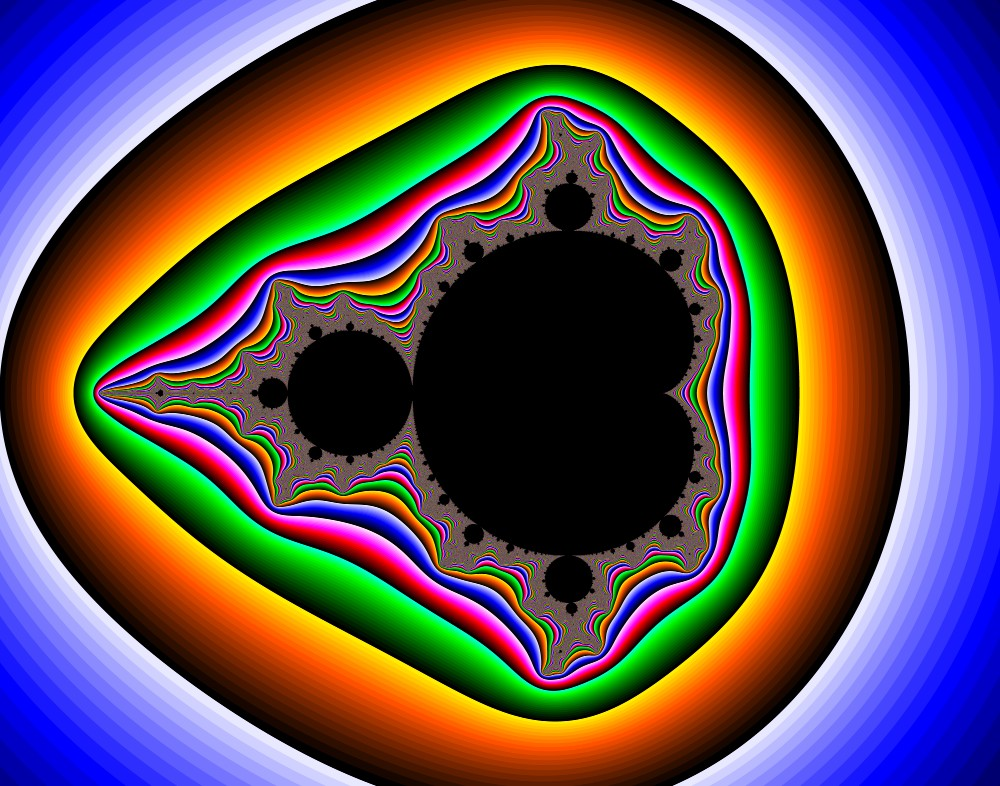
\includegraphics[width=0.38\textwidth]{pictures/apfel}
  \end{center}
\caption{Apfelmännchen}
\vspace{10pt}
\end{wrapfigure}
Wir haben die imaginäre Einheit $\mathrm{i}$ definiert als L\"osung der Gleichung
$$x^2 = -1.$$
Warum sollten wir nicht ähnlich bei anderen Gleichungen vorgehen, die im Reellen keine L\"osung besitzen?
\begin{bsp}
Als Beispiel betrachten wir die Gleichung
$$x \cdot 0 = 1.$$
Diese Gleichung besitzt keine L\"osung in $\mR$, denn das Produkt einer reellen Zahl mit $0$ ist immer $0$.

Analog zu unserem Vorgehen bei der Definition der imaginären Einheit definieren wir nun eine Zahl $j$, die eine L\"osung der obigen Gleichung sein soll. Es soll also gelten
$$j\cdot 0=1.$$
Mit dieser Zahl $j$ soll man nach den \"ublichen Regeln rechnen k\"onnen (Permanenzprinzip). Dann gilt zum Beispiel:
$$(0+0)\cdot j=0\cdot j=1.$$
Es ist aber auch
$$(0+0)\cdot j=0\cdot j+0\cdot j=1+1=2.$$
Das heisst $1=2$ und widerspricht dem Rechnen in $\mR$. Also gibt es in $\mR$ keine sinnvolle Erweiterung, in der die Gleichung $x\cdot0=1$ eine L\"osung besitzt.
\end{bsp}
Wir haben Gl\"uck, dass es mit $\mathrm{i}$ so gut funktioniert! Und vielleicht verstehen Sie jetzt auch, warum so viele Mathematiker und Mathematikerinnen sich so lange mit den imaginären Zahlen schwer getan haben. Man konnte ja nie wissen, ob man nicht irgendwann auf einen Widerspruch st\"osst!
\begin{ueb}[gleich $0$]
Zeige, dass die Gleichung
$$10^x=0$$
keine reelle L\"osung haben kann.
\end{ueb}

\section{i ist nicht die Wurzel aus -1}

In vielen Lehrb\"uchern findet man die Schreibweise $\mathrm{i} = \sqrt{-1}$. Was ist problematisch an dieser Schreibweise?
Wenn man $\mathrm{i} = \sqrt{-1}$ schreibt, dann ist man nat\"urlich auch in Versuchung, die \"ublichen Rechenregeln f\"ur Wurzeln von $\mR$ auf $\mC$ zu \"ubertragen. Das f\"uhrt allerdings zu Schwierigkeiten. Die Wurzelrechnung ist im Komplexen etwas komplexer.

\begin{bsp}
Verwendet man in $\mC$ die \"ublichen Wurzelregeln aus $\mR$, dann erhält man
$$
-1=\mathrm{i}^2=\sqrt{-1}\cdot\sqrt{-1}=\sqrt{(-1)\cdot(-1)}=\sqrt{1}=1.
$$
$-1=1$ steht offensichtlich im Widerspruch zum Rechnen in $\mR$. Die Schreibweise $\mathrm{i}=\sqrt{-1}$ ist deshalb irref\"uhrend und sollte nicht verwendet werden.
\end{bsp}

\begin{ueb}[Wurzeln]
Überlege dir, wo in der obigen Rechnung der Fehler stecken muss. Welche Operation ist demnach in $\mC$ nicht erlaubt?
\end{ueb}

\section{Ist i positiv oder negativ?}

Aus dem Reellen wissen Sie: Eine von null verschiedene, reelle Zahl ist entweder positiv oder negativ. Überdies gilt: Reelle Zahlen lassen sich der Gr\"osse nach ordnen.

Wie stehst mit $\mathrm{i}$? Sicher ist $\mathrm{i}\neq0$, denn $0^2=0$, aber $\mathrm{i}^2=-1$. Also kommt $\mathrm{i}>0$ oder $\mathrm{i}<0$ in Frage. Nehmen wir an, dass $\mathrm{i}>0$. Durch Multiplikation dieser Ungleichung mit $\mathrm{i}$ folgt
$$\mathrm{i}^2>0,$$
wobei das Ungleichheitszeichen wegen der Annahme $\mathrm{i}>0$ unverändert bleibt. Also haben wir $-1>0$, was im Widerspruch zum Rechnen in $\mR$ steht. Dann m\"usste also $\mathrm{i}<0$ gelten?

\begin{ueb}[Ordnung geht verloren]
Zeige, dass $\mathrm{i}<0$ auch nicht sein kann.
\end{ueb}

\begin{bem}
Die Zahl $\mathrm{i}$ ist also weder positiv noch negativ.
\end{bem}

Die Erweiterung von $\mR$ zu $\mC$ wird also mit dem Verzicht auf Ordnung bezahlt. In $\mC$ gelten die Anordnungsaxiome nicht mehr.

\section{Die logarithmische Spirale}
\begin{wrapfigure}{r}{0.3\textwidth}
\begin{center}
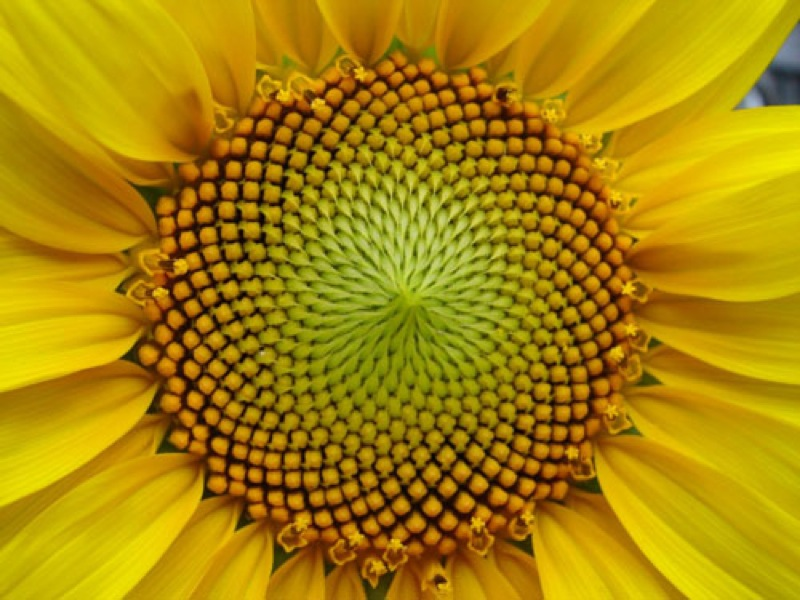
\includegraphics[width=0.3\textwidth]{pictures/sonnenblume}
\end{center}
\caption{Sonnenblume und logarithmische Spirale}
\end{wrapfigure}
In der Natur und im Alltag kommen eine Vielzahl von Spiralformen vor. Die Kerne von Sonnenblumen sind spiralf\"ormig um den Mittelpunkt angeordnet, Schneckenhäuser wachsen spiralf\"ormig, Luftschlangen sind als Spirale aufgewickelt.
\begin{ueb}[Spiral]
Es sei
$$z=1+\mathrm{i}.$$
Berechne $z^2,z^3,\dots,z^8$ und zeichne die entstehenden Zahlen zusammen mit $z$ als Punkte in ein Koordinatensystem. Verbinde anschliessend die Punkte durch Strecken.
\end{ueb}
\noindent Was Sie erhalten ist bereits eine Annäherung an eine logarithmische Spirale. Eine vollständige logarithmische Spirale erhält man, wenn man von den diskreten Exponenten $1, 2,\dots, 8$ zu einem kontinuierlichen Exponenten $t \in \mR$ \"ubergeht. Statt $z^1,z^2,\dots$ betrachten wir $z^t$ mit $t\in\mR$.

\begin{center}
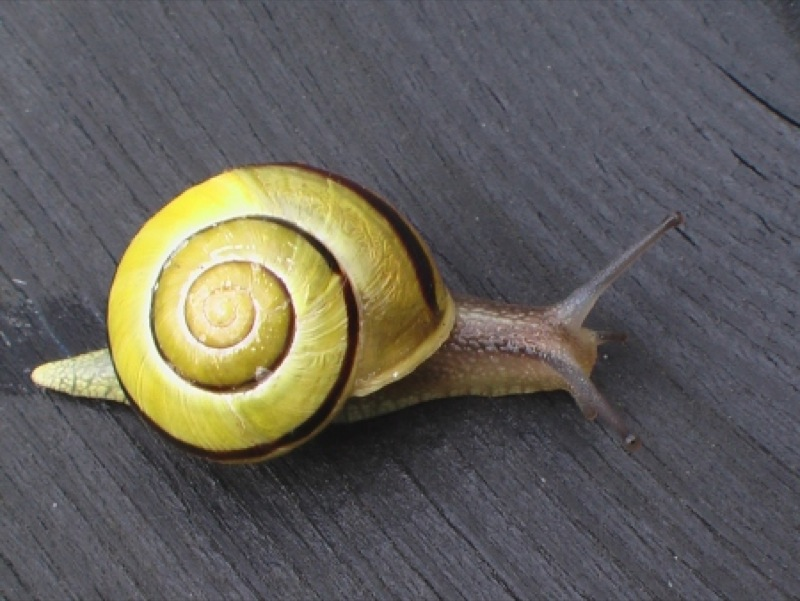
\includegraphics[width=0.45\textwidth]{pictures/schneckenhaus}
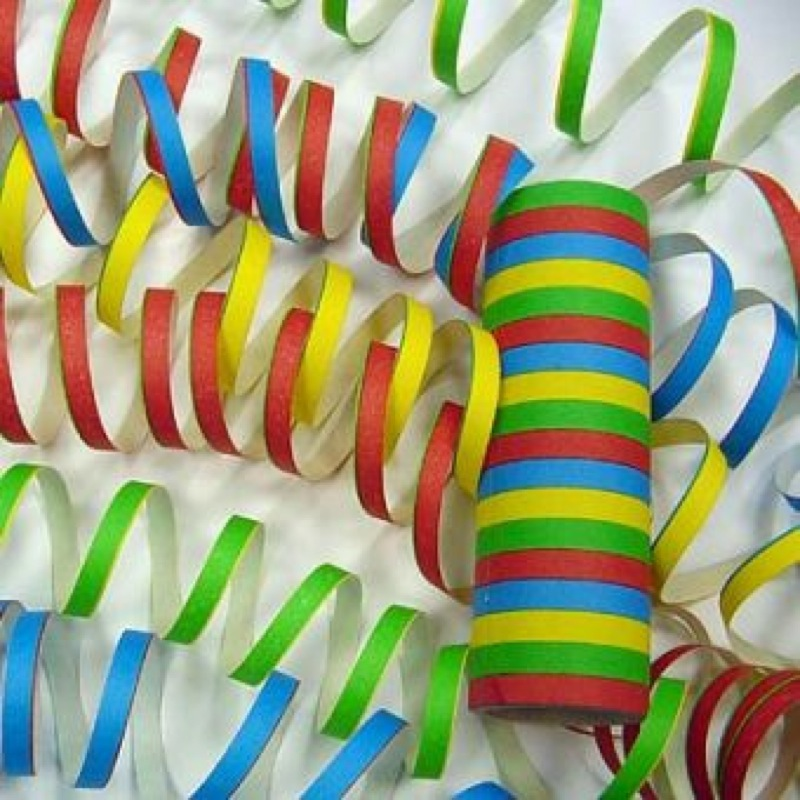
\includegraphics[width=0.338\textwidth]{pictures/luftschlange}
\end{center}

\begin{bsp}
Wir betrachten
$$1+\mathrm{i}=\sqrt{2}e^{\mathrm{i}\frac{\pi}{4}}$$
kontinuierlich. Es ist
$$(1+\mathrm{i})^t=\left(\sqrt{2}\mathrm{e}^{\mathrm{i}\frac{\pi}{4}}\right)^t=2^\frac{t}{2}\cdot \mathrm{e}^{\mathrm{i}\frac{\pi}{4}t}=:w(t).$$
Zu jedem Wert $t$ kann die Zahl $w(t)$ bestimmt werden und der zugeh\"orige Punkt in der Gauss'schen Zahlenebene eingezeichnet werden. Alle diese Punkte bilden eine Spirale, eine so genannte \textbf{logarithmische Spirale}
\begin{center}
%\includegraphics[width=0.45\textwidth]{geogebra/spirale.pdf}

\begin{tikzpicture}[line cap=round,line join=round,>=triangle 45,x=0.2cm,y=0.2cm]
\draw[->,color=black] (-16.93,0) -- (17.54,0);
\foreach \x in {-15,-10,-5,5,10,15}
\draw[shift={(\x,0)},color=black] (0pt,2pt) -- (0pt,-2pt) node[below] {\footnotesize $\x$};
\draw[color=black] (16.63,0.24) node [anchor=south west] {$x$};
\draw[->,color=black] (0,-16.02) -- (0,16.63);
\foreach \y in {-15,-10,-5,5,10,15}
\draw[shift={(0,\y)},color=black] (2pt,0pt) -- (-2pt,0pt) node[left] {\footnotesize $\y$};
\draw[color=black] (0.27,15.45) node [anchor=west] {$y$};
\draw[color=black] (0pt,-10pt) node[right] {\footnotesize $0$};
\clip(-16.93,-16.02) rectangle (17.54,16.63);
\draw[smooth,samples=1000,domain=-12.566370614359172:12.566370614359172] plot[parametric] function{2**(t/2)*cos((0.79*t)),2**(t/2)*sin((0.79*t))};
\end{tikzpicture}

\end{center}
\end{bsp}

\begin{ueb}[Spirale im Kleinen]
Überlege dir, wie die logarithmische Spirale in einer Umgebung von $0$ aussieht.
\end{ueb}

Auf den ersten Blick erscheint es sinnvoll, die folgende Vorschrift zu verwenden:
Wenn $z$ eine nicht reelle Zahl ist, dann betrachten wir die Kurve $w(t)=z^t,\q t\in\mR.$

\begin{ueb}[versandet]
Was passiert, wenn man $z = \mathrm{i}$ wählt? Welche anderen komplexen Zahlen verwendet man demnach auch nicht, um eine logarithmische Spirale zu erzeugen?
\end{ueb}

\begin{cdef}[Logarithmische Spirale]{def:logspiral}
Es sei $z$ eine nicht reelle Zahl mit $\abs{z}\neq1$. Die durch die Gleichung
$$w(t)=z^t,\q t\in\mR,$$
gegebene Kurve heisst \emph{logarithmische Spirale}.
\end{cdef}

\begin{bem}
Es gab einen Mathematiker, der von der logarithmischen Spirale so begeistert war, dass er sie in seinen Grabstein gemeisselt haben wollte. Dass sein Wunsch nicht erf\"ullt wurde, ist noch heute im Baseler M\"unster zu sehen. Welche Spirale \textsc{Jakob Bernoullis} Grabstein ziert und warum k\"onnen Sie beispielsweise in dem Buch von \textsc{Johanna Heitzer} nachlesen. Dort finden Sie auch eine Erkl\"arung, warum man diese Art von Spirale \glqq logarithmisch\grqq\ nennt. Alternativ dazu k\"onnen Sie unter \glqq Jakob Bernoulli\grqq\ und \glqq logarithmische Spirale\grqq\ im Internet recherchieren.
\end{bem}

\section{Mathematische Motten}

Dass Motten und andere Nachtfalter von starken Lichtquellen angezogen werden, weiss jeder, der einmal im Sommer mit einer Lichtquelle im Freien gesessen hat oder sich im Freiluftkino \"uber die Insektenschatten auf der Leinwand ärgern musste. Entomologen benutzen diese Tatsache beim so genannten Lichtfang.
Warum ist das aber so? Wussten Sie, dass Motten auch von Lichtquellen abgestossen werden k\"onnen? Und was hat das Ganze eigentlich mit logarithmischen Spiralen zu tun?

Warum Motten vom Licht angezogen werden, ist noch nicht vollständig geklärt. Die plausibelste Theorie nimmt an, dass Motten sich bei ihren nächtlichen Fl\"ugen an nat\"urlichen Lichtquellen orientieren. Der Mond oder auch helle Sterne bilden eine solche Lichtquelle.
Man nimmt an, dass Motten geradeaus fliegen, indem sie zu den Lichtstrahlen dieser Lichtquellen einen konstanten Flugwinkel einhalten. Da der Mond nämlich sehr weit entfernt ist, sind die Lichtstrahlen, die von ihm bei uns auf der Erde ankommen, in guter Näherung Parallelen. Wenn die Motte also einen konstanten Winkel zu ihnen einhält, fliegt sie automatisch geradeaus.
Das Mondlicht fällt schräg von links oben ein. Die Motte fliegt mit dem konstanten Flugwinkel $\ga$ zu diesem Mondlicht.
Was passiert nun, wenn sich eine helle Lichtquelle wie etwa eine Kerze oder eine Lampe in der Nähe befindet?
Wir nehmen idealisiert an, dass diese Lichtquelle punktf\"ormig ist.
\begin{ueb}[Motte]\label{ueb:motte}
Zeichne die Flugbahn der Motte in eine Skizze ein. Ber\"ucksichtige dabei, dass die Motte zu den Lichtstrahlen stets den konstanten Flugwinkel $\ga$ einhält.
\end{ueb}
Bei der Bearbeitung der vorangegangenen Aufgabe \ref{ueb:motte} haben Sie festgestellt, dass sich die Motte spiralf\"ormig auf die Lichtquelle zubewegt.
Die Form der Spirale sollte Ihnen bekannt vorkommen. Es handelt sich um eine logarithmische Spirale.
Logarithmische Spiralen haben nämlich die Eigenschaft, dass sie jede vom Ursprung ausgehende Gerade immer unter dem gleichen Winkel schneiden. In unserem Beispiel sind die vom Ursprung ausgehenden Geraden die Lichtstrahlen der k\"unstlichen Lichtquelle. Die logarithmische Spirale ist die Flugbahn der Motte.

\section{Juliamengen}

Wahrscheinlich haben Sie schon solche Bilder gesehen oder den Namen geh\"ort: Seit man Juliamengen auf dem Computer berechnen kann, sind Postkarten und Poster von den farbig schillernden Gebilden sehr beliebt.

Wir beginnen mit einem einfachen Rezept. Sie k\"onnten dieses Rezept beispielsweise einem Computer einprogrammieren. Es lautet folgendermassen:
\begin{enumerate}
\item Nimm eine komplexe Zahl. (Diese Zahl nennen wir den \emph{Startwert}.)
$$z_0=c$$
\item Quadriere diese Zahl und subtrahiere $1$ von der quadrierten Zahl.
$$z_1=c^2-1$$
\item Nimm die so entstandene neue Zahl und wiederhole die Schritte $2.$ und $3.$ bis in alle Unendlichkeit\dots
$$z_{k+1}=z_k^2-1,\q z_0=c$$
\end{enumerate}
\begin{bem}
Wenn Sie dieses Rezept wirklich programmieren wollten, m\"ussten Sie nat\"urlich noch eine Abbruchbedingung einbauen. Beispielsweise k\"onnten Sie eine Anweisung schreiben \glqq H\"ore nach tausend Wiederholungen auf\grqq. Sonst läuft das Programm unendlich lange.
\end{bem}

\begin{bsp}
Als Startwert nehmen wir die Zahl $2$. Wir schreiben $z_0 = 2$. Damit dr\"ucken wir aus, dass $2$ der Startwert unserer Zahlenfolge ist.
Nach dem Rezept sollen wir $2$ nun quadrieren und anschliessend $1$ abziehen. Dadurch erhalten wir $2^2 - 1 = 4 - 1 = 3$. Diesen neuen Wert nennen wir $z_1$. Es ist also $z_1 = 3$.
Gemäss dem Rezept sollen wir nun wieder den zweiten und dritten Schritt ausf\"uhren, diesmal mit der Zahl $3$ statt $2$. Wir erhalten $3^2 -1 = 9-1 = 8$. Diese Zahl nennen wir $z_2$. Es ist also $z_2 = 8$.
Wir k\"onnen nun immer weiter fortfahren und erhalten neue Zahlen $z^3, z^4, z^5$, usw. Insgesamt erhalten wir eine Zahlenfolge $z_0, z_1, z_2, z_3, z_4, z_5,\dots$.
\end{bsp}
\begin{ueb}[Folge] \label{ueb:folge}
Berechne mit dem TR die Folgeglieder $z_3$ bis $z_6$.
\end{ueb}
Wir k\"onnen die Zahlenfolge, die auf diese Weise entsteht, durch eine Rechenvorschrift angeben:
$$z_0=2,\q z_{k+1}=z_k^2-1\q\forall n\geq0.$$
Wie Sie in †bung \ref{ueb:folge} gesehen haben, werden bei der Folge oben die Folgeglieder immer gr\"osser. Ist das immer so? Was passiert, wenn wir statt $2$ einen anderen Startwert $z_0$ wählen?

\begin{ueb}[Startwerte]\label{ueb:folgen}
Berechne f\"ur folgende Startwerte $z_1$ bis $z_4$.\\

(a) $z_0=0\q$ (b) $z_0=1+\mathrm{i}\q$ (c) $z_0=\frac{1}{2}$
\end{ueb}

\begin{ueb}[Beträge]
Berechne zu den Zahlenfolgen aus Übung \ref{ueb:folgen} die Folge der Beträge.
\end{ueb}

Bei dem ersten Beispiel ist der Fall klar: Die Beträge wechseln immer zwischen $0$ und $1$. Bei dem zweiten Beispiel ist das Verhalten nicht ganz so klar. Aber immerhin scheint es so zu sein, dass die Beträge immer gr\"osser werden. Dass das tatsächlich der Fall ist, m\"usste man nat\"urlich beweisen. Wir wollen uns hier aber mit der Vermutung zufrieden geben, dass es so ist. Bei dem dritten Beispiel scheint es so zu sein, dass die Beträge immer kleiner als $1$ bleiben. Das ist tatsächlich so. †berlegen Sie sich einmal, warum das so ist.

\begin{figure}
\begin{center}
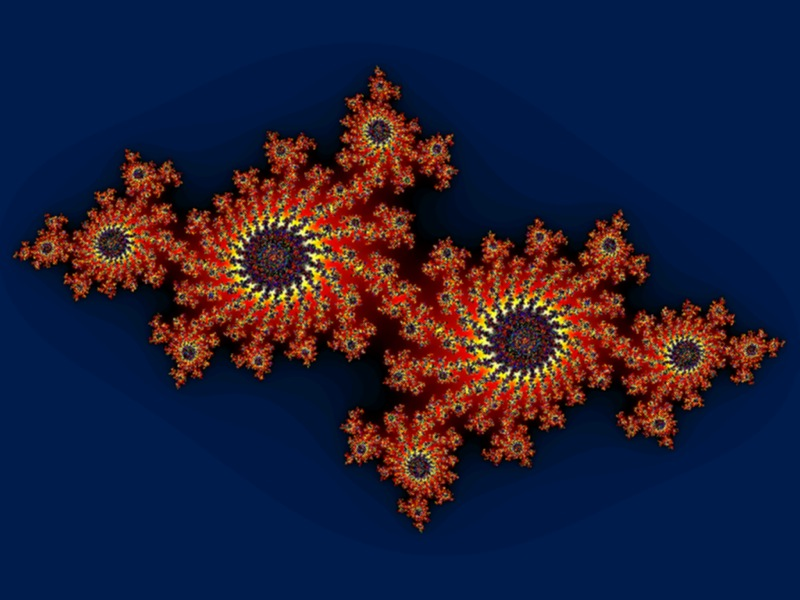
\includegraphics[width=0.618\textwidth]{pictures/julia1}
\end{center}
\caption{Eine Juliamenge}
\end{figure}

Wenn Sie weitere Startwerte wählen, werden Sie feststellen, dass Sie neue Folgen erhalten, die sich verschieden verhalten. Manche pendeln zwischen einigen wenigen Werten hin und her, manche werden betragsmässig immer gr\"osser, und bei manchen scheinen die Beträge der Zahlen einen bestimmten Wert nie zu \"uberschreiten, selbst wenn sie nicht nur zwischen zwei Werten hin und her schwanken. Im nächsten Abschnitt wollen wir das ausnutzen, um eine Juliamenge zu erhalten.

Wir benutzen nun unsere Zahlenfolgen, um die Punkte der Gauss'schen Zahlenebene auf eine bestimmte Art und Weise zu färben. Dabei gehen wir nach folgendem Schema vor:
Wir nehmen eine komplexe Zahl $z_0$ in der Gauss'schen Zahlenebene. Diese Zahl nehmen wir als Startwert f\"ur eine Folge von Zahlen, die nach dem oben beschriebenen Rezept berechnet wird. Jetzt färben wir den Punkt $z_0$ in der Gauss'schen Zahlenebene entweder schwarz oder weiss. Und zwar entscheiden wir nach folgendem Kriterium:
Wachsen die Beträge der (theoretisch unendlich vielen) Zahlen in der Folge \"uber alle Grenzen, so färben wir den Punkt schwarz. Andernfalls färben wir den Punkt weiss.
Nach und nach f\"uhren wir dies mit allen Punkten der Gauss'schen Zahlenebene durch. Wir erhalten so ein schwarz-weisses Muster. Alle weissen Punkte in der Ebene zusammen sind eine Juliamenge! Und so sieht sie aus:

\begin{center}
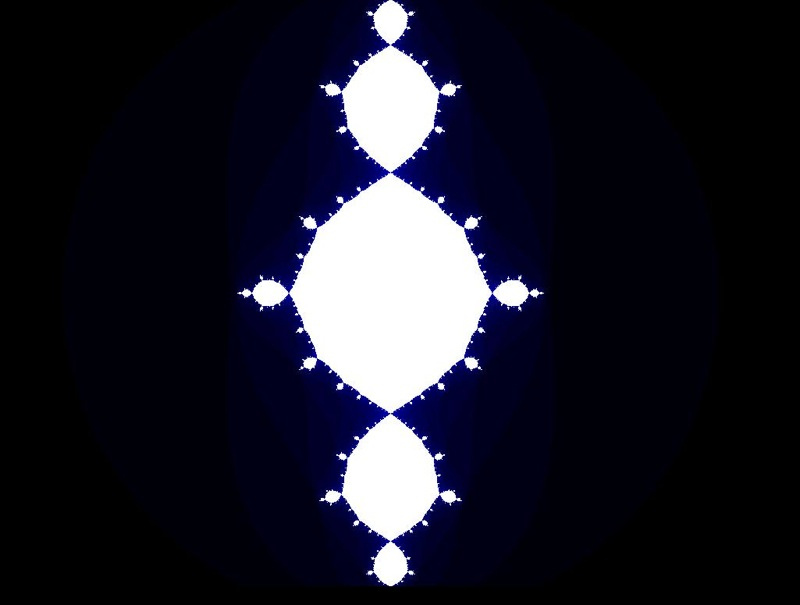
\includegraphics[width=0.382\textwidth, angle= 90]{pictures/julia2}
\end{center}

Die reelle und imaginäre Achse haben wir weggelassen. Schliesslich geht es uns nur um das Prinzip --- wir wollen nicht genau berechnen, wo die Randpunkte auf den Achsen liegen. Das ist \"ubrigens auch gar nicht so einfach.

\subsection{Weitere Juliamengen}

Es gibt nicht nur eine Juliamenge, sondern unendlich viele verschiedene.
Sehen wir uns doch noch einmal die Rechenvorschrift an, die zu unserer Juliamenge geh\"ort. Zu einem Startpunkt $z_0$ haben wir die Folgenglieder der zugeh\"origen Folge berechnet durch
$$z_{k+1}=z_k^2-1\q\forall n\geq0.$$
Wir haben von dem Quadrat eines Folgenglieds immer $1$ abgezogen. Oder anders
ausgedr\"uckt: $-1$ dazu addiert.
Jetzt wollen wir die Rechenvorschrift ein wenig abändern: Wir addieren nicht
mehr $-1$ dazu, sondern $\frac{1}{2}\mathrm{i}$. Warum auch nicht? Wir berechnen dann zu einem Startpunkt $z_0$ die Folgenglieder der zugeh\"origen Folge durch die Vorschrift
$$z_{k+1}=z_k^2+\frac{1}{2}\mathrm{i}\q\forall n\geq0.$$
Danach gehen wir ganz genauso vor wie im ersten Beispiel: Wir färben einen Punkt der Ebene schwarz, wenn die Beträge der zugeh\"origen Folgenglieder \"uber alle Grenzen anwachsen, und andernfalls weiss. Dadurch erhalten wir wieder eine Juliamenge. Sie sieht so aus:

\begin{center}
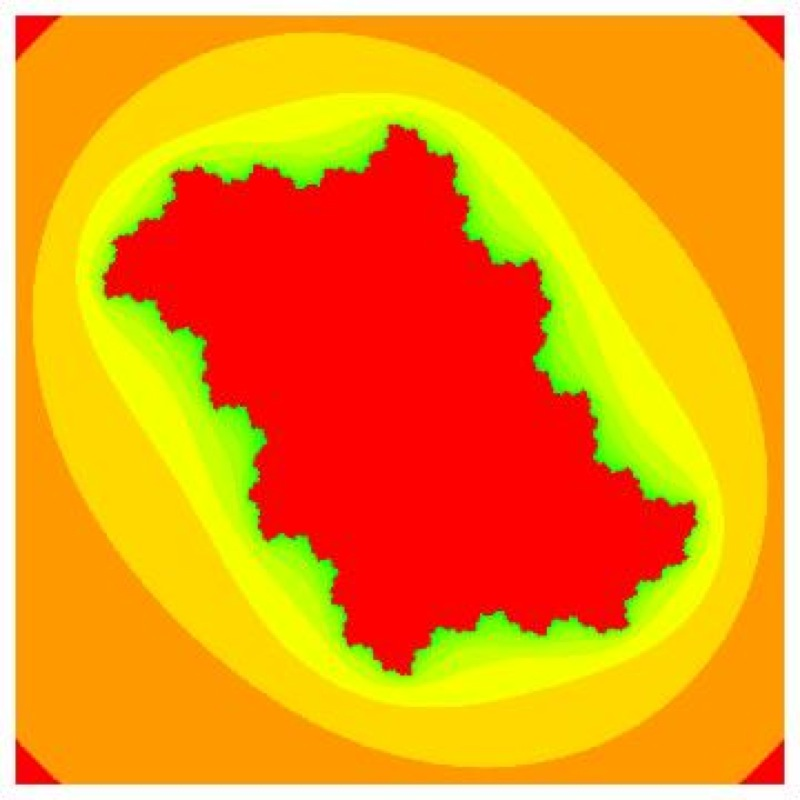
\includegraphics[width=0.618\textwidth]{pictures/julia3}
\end{center}

\begin{bem}
Dieses Bild wurde mit Mathematica erzeugt:

\begin{lstlisting}
Julia[zo_] := 
  Module[{z = zo, i = 0}, 
   While[i < 100 && Abs[z] < 2,
   z = z^2 + c; i++]; i]; c = 0.5*I;
   DensityPlot[Sqrt[Julia[x + I y]],
   {x, -1.5, 1.5}, {y, -1.5, 1.5}, 
 PlotPoints -> 275, Mesh -> False,
 Frame -> False,
 ColorFunction -> Hue]
\end{lstlisting}
\end{bem}

Auf diese Weise k\"onnen wir unendlich viele Juliamengen erzeugen. Die allgemeine Formulierung der Rechenvorschrift, mit der wir zu einem Startpunkt $z_0$ die Folgenglieder der zugeh\"origen Folge berechnen, lautet
$$z_{k+1}=z_k^2+c,\q\forall n\geq0,$$
wobei $c$ eine komplexe Zahl sein soll. F\"ur jede komplexe Zahl $c$ erhalten wir eine
Juliamenge. Wie die Mengen f\"ur $c = -1$ und f\"ur $c = \frac{1}{2}\mathrm{i}$ aussehen, haben wir schon gesehen.

Bilder von Juliamengen sind deshalb so beliebt, weil sie bunt sind und sch\"on aussehen. Was haben eigentlich die schwarz-weissen Muster mit diesem Farbenrausch zu tun?
Das ist nur eine von vielen Fragen, denen wir hier nicht mehr nachgehen. Genau wie die Frage, wie Sie denn nun selbst Bilder von Juliamengen auf dem Computer erzeugen k\"onnen, oder woher der Name \glqq Juliamenge\grqq\ kommt. Und was ist mit der \emph{Mandelbrotmenge}? Die taucht doch im Zusammenhang mit Juliamengen auch immer wieder auf. Und was haben Juliamengen mit Fraktalen zu tun?

\cleardoublepage
\listoffigures
\listoftables
%\newpage
%\nocite{*}
%\bibliographystyle{plain}
%\bibliography{preamble/literaturgoogle}
\end{document}